% Preamble
\documentclass[11pt, oneside]{article}   	%standardeinstellung
\usepackage{amsmath}				%damit du formeln eingeben kannst
\usepackage[parfill]{parskip}    			% neuer absatz durch leere zeile
\usepackage{graphicx}				% bilder einfügen
\usepackage[onehalfspacing]{setspace}	%1,5 facher zeilenabstand
\usepackage{hyperref}				%damit man links erstellen kann
\usepackage{float}					%intelligentes anpassen von bildern, damit es keine lücken im text gibt
\graphicspath{ {figures/} }				%automatisches erstellen von "List of Figures"
\usepackage[font=small,labelfont=bf]{caption} %formatierung der bildunterschrift
 \usepackage{geometry}				%Seitenlayout
 \usepackage{tikz}
 \usetikzlibrary{shapes,arrows}

 \geometry{						%musst du nicht unbedingt selbst einstellen
 a4paper,
 total={210mm,297mm},
 left=15mm,
 right=15mm,
 top=25mm,
 bottom=20mm,
 }

\usepackage{ragged2e}
\usepackage[export]{adjustbox}
\usepackage{dsfont}
\usepackage{amssymb}
\usepackage{caption}
\usepackage{natbib}
\usepackage[utf8]{inputenc}
\usepackage{amsmath}
\usepackage{amsfonts}
\usepackage{amssymb}
\usepackage{wrapfig}
\usepackage{subcaption}
\usepackage{pdflscape}
\usepackage{filecontents,url}
\usepackage{soul}
\usepackage[space]{grffile}
\usepackage[UKenglish]{isodate}
\usepackage{anyfontsize}
\def\one{\mbox{1\hspace{-4.25pt}\fontsize{12}{14.4}\selectfont\textrm{1}}} % 11pt

\let\oldref\ref
\renewcommand{\ref}[1]{(\oldref{#1})}


\title{Spatial Inefficiencies in Africa's Trade Network}
\author{Tilman Graff -- University of Oxford}
\date{\today}

\begin{document}

\bibliographystyle{cantoni_copy}
\maketitle
\begin{abstract}
  Are African roads where they should be? I assess the efficiency of transport networks for every country in Africa. Using rich data from satellites and online routing services, I simulate optimal trade flows through more than 90,000 links for the entire continent. Employing a recently established framework from the optimal transport literature, I maximise over the space of networks to find the optimal road system for every country. Where would the social planner ideally build more roads and which roads are superfluous in promoting beneficial trade? Comparing current and optimal network, I then construct a novel dataset of local network inefficiency for more than 10,000 African regions. I analyse roots of the substantial variation present in this measure. I find that colonial infrastructure projects from more than a century ago still persist in significantly skewing trade networks towards a sub-optimal state. Areas close to colonial railroads are about 1.7\% too well off given their position in the network.
\end{abstract}

% End Preamble

%-------------------------------------------------

\section{Introduction}

\section{A model of Optimal Transport Networks}

Are African roads where they should be? To gain a notion of transport network efficiency, the first step is to identify the optimal allocation of roads for a given country. If a social planner were to observe a country's geography, where would she place highways and footpaths, and which regions would she leave unconnected? Intuitively, this optimal network should succeed in connecting regions with a heavy interest in beneficial trade, place roads only where they are cheap to build, and avoid overspending on roads that nobody ever uses.

Optimising over the space of possible network has proven to be challenging to researchers and policymakers alike. The many contingencies and non-linearities of the network structure make it hard to obtain a unique closed-form solution to the problem. The large number of possible connections between locations have, furthermore, led to computational challenges. Researchers and practitioners have hence often been left only with slow, iterative algorithms to obtain a notion of local network optimality. A recent contribution by \cite{fajgelbaum_optimal_2017}, however, manages to circumvent these issues. Under a number of reasonable assumptions, it paves the way for obtaining closed-form solutions to the problem of optimal transport networks without straining computational capabilities all too much. It thereby allows for nesting many of the standard models of the trade literature and can thus flexibly be tailored to the question at hand. This thesis harnesses a version of the \citeauthor{fajgelbaum_optimal_2017} framework to compute the optimal transport network for every African country. The model is introduced in the following paragraphs, chapter \eqref{chapter:calibration} then describes the procedure used to bring the model to the data.

\subsection{Geography}

Following the set-up and notation of \cite{fajgelbaum_optimal_2017}, I consider a set of locations $\mathcal{I} =\{ 1,...,I\}$. Each location $i \in \mathcal{I}$ inhabits a number of homogeneous consumers $L_{i}$. This number is treated as given and fixed for every location, such that consumers are not allowed to move between locations. Each consumer has an identical set of preferences characterised by
\begin{equation*}
  u = c^{\alpha}
\end{equation*}
where $c$ denotes per capita consumption. Due to the symmetry of consumers in every location, per capita consumption (and therefore utility) is identical for every consumer within each location, such that every consumer in location $i$ consumes $c_{i}$. It is sensible to further denote
\begin{equation*}
  C_{i} = L_{i}c_{i}
\end{equation*}
as total consumption in location $i$.

There there is a set of goods $\mathcal{N}$ denoted by $n =\{ 1,...,N\}$. Total consumption in each location is defined as the CES aggregation of these goods
\begin{equation*}
  C_{i} = \bigg( \sum_{n=1}^{N} (C_{i}^{n})^{\frac{\sigma-1}{\sigma}}\bigg)^{\frac{\sigma}{\sigma-1}}
\end{equation*}
where $\sigma$ denotes the standard elasticity of substitution and $C_{i}^{n}$ denotes the supply of good $n$ in location $i$. Locations specialise in the production of goods such that each location only supplies one variety $n \in \mathcal{N}$. Let
\begin{equation*}
  Y_{i} = Y_{i}^{n}
\end{equation*}
denote the total production output of location $i$.\footnote{Note how this assumption does not normally coincide with perfect specialisation in the sense that every good is only produced in one location \citep[as in e.g.][]{Anderson_Gravitygravitassolution_2003}. This \emph{Armington} assumption is only satisfied if $N=I$ (and every good being produced).} In contrast to \citeauthor{fajgelbaum_optimal_2017}, my version of the model takes output levels as given and hence does not take a stand on how the output is produced. It is conceivable to think of a production function in which consumers produce goods themselves or an environment in which capital does the work for them. Importantly, however, by remaining agnostic about the production process, output levels are treated as fixed throughout the analysis. The only assumption about the supply side of the economy is perfect specialisation on one of the goods, which does not allow locations to choose between different production opportunities.

\subsection{Network Topography}
Locations $\mathcal{I}$ can be conceived as representing the nodes of an undirected network graph. Each location $i$ is directly connected to a set of neighbours $N(i) \in \mathcal{I} \setminus \{ i\}$. I consider locations to lie on a two-dimensional rectangular grid where each node is connected to its eight surrounding nodes to the North, North-East, East, and so on. Nodes at the border of the network graph might have fewer than eight neighbours. Let $\mathcal{E}$ denote the set of edges connecting neighbouring nodes and note that $(\mathcal{I}, \mathcal{E})$ fully describes the underlying network topography.\footnote{While I follow the notation of \cite{fajgelbaum_optimal_2017}, the set up so far is very similar to many of the recent contributions in the theory of trade in networks, like \cite{allen_welfare_2016} or \cite{Galichon_OptimalTransportMethods_2016}.}

All goods can be traded within the network. Let $Q_{i,k}^{n}$ denote the total flow of good $n$ travelling between nodes $i$ and $k \in N(i)$. The network affects trade flows in the sense that goods can only be shipped between neighbouring nodes. However, nothing prevents goods to travel far distances through the network by passing multiple locations after each other. To send a good on to a far away destination, the optimal trade route will potentially make multiple stop-overs in intermediate locations. The entire flow-topography of the trade network can hence be modelled simply by considering flows between neighbouring nodes.

Shipping goods from location $i$ to location $k \in N(i)$ incurs trade costs, which are modelled in the canonical iceberg form. In order for 1 unit of good $n$ to arrive at location $k$, origin location $i$ has to send $(1+\tau_{i,k}^{n})$ units on its way. $\tau_{i,k}^{n}$ can be understood as a tax on transport, causing a fraction of goods to not arrive in the destination location. This iceberg formulation has analytical advantages, as it makes modelling an entire transport sector superfluous. Importantly, barriers to trade are the dimension through which geography is introduced to the model. It is now costly for goods to travel elaborate and long routes through the network and notions of distance and connectedness start to play a role. The main assumption in \citeauthor{fajgelbaum_optimal_2017}'s derivation of optimal networks is then about the functional form of $\tau_{i,k}^{n}$. In particular, the authors model iceberg trade costs for shipping good $n$ between neighbouring locations $i$ and $k$ as
\begin{equation}
  \tau_{i,k}^{n} = \delta^{\tau}_{i,k} \frac{(Q_{i,k}^{n})^{\beta}}{I_{i,k}^{\gamma}}
  \label{eq:tau}
\end{equation}
where $I_{i,k}$ is defined as the level of \emph{infrastructure} on the edge between nodes $i$ and $k$. Since model parameters are restricted at $\delta^{\tau}_{i,k}, \beta, \gamma >0$, more infrastructure on a given link decreases the cost of trading between them. $I_{i,k}$ will later be calibrated more succinctly, but for now it suffices to picture anything that might make trade costs between two locations smaller, like broader and better roads, less detours or faster train tracks. In a first-best scenario, infrastructure between all nodes would be set infinitely high to wash away all trade costs and enable goods to travel seamlessly through the entire network. As $I_{i,k}$ is independent from $n$, higher infrastructure between two nodes will benefit the trade of all goods travelling on this edge. $\delta^{\tau}_{i,k}$ is a scaling parameter, which allows trade costs to be flexibly adjusted for any given origin-destination pair. Note that $\delta^{\tau}_{i,k}$ is also  independent of good $n$. In later calibrations, the main component of $\delta^{\tau}_{i,k}$ will be the geographical distance between locations $i$ and $k$. Distance is thought to increase trade costs independently from infrastructure provision on the travelled link.

The strongest assumption of the \citeauthor{fajgelbaum_optimal_2017} framework is the dependence of trade costs on $Q_{i,k}^{n}$, the total flow of goods on the link. Higher existing trade volumes on any given edge make sending an additional good more costly, a dynamic the authors refer to as \emph{congestion}. A few things are worth noting about this assumption. First, congestion plays the role of an externality in the trade network. Sending one additional unit of goods from $i$ to $k$ makes all other existing shipments more expensive. The social planner realises this and takes congestion into account when determining optimal trade flows.\footnote{Perhaps not surprisingly, the existence of a negative externality will lead to over-provision of trade in the decentralised market solution to the problem. In their technical appendix \citeauthor{fajgelbaum_optimal_2017} demonstrate how a moderately straightforward transport tax can internalise the externality and establish the applicability of the two welfare theorems. As this thesis stays in the social-planner conception of the problem, such decentralisation conditions are of minor concern going forward.} Second, congestion forces \emph{are} allowed to vary with different goods. While analytically appealing, this assumption might strike the reader as odd at first. Congestion for transporting some good $n$ is only caused by existing trade flows of the same good. No matter how many other goods are being pushed through an edge, each one only causes congestion nuisances for other shipments of the same variety. While \citeauthor{fajgelbaum_optimal_2017} demonstrate a way to circumvent this peculiarity of the model, as will be discussed soon the assumption has clear analytical advantages and is hence kept for the purpose of this thesis.

In equilibrium, each location cannot consume and export more than it produced and imported. More formally
\begin{equation}
  C_{i}^{n} + \sum_{k\in N(i)}^{}Q_{i,k}^{n}(1+\tau_{i,k}^{n}(Q_{i,k}^{n}, I_{i,k})) \leq Y_{i}^{n} + \sum_{j\in N(i)}^{}Q_{j,i}^{n}
  \label{eq:balanced_flows}
\end{equation}
must hold for every $n$ and $i$. Equation \eqref{eq:balanced_flows} is a variation of what \citeauthor{fajgelbaum_optimal_2017} call the \emph{Balanced Flows Constraint}.

\subsection{Optimal Infrastructure Provision}
So far, we have merely cast a plain model of trade in a geographical network, albeit with a slightly unconventional trade cost functional. Solving this model is more or less straightforward and would result in trade flows caused by heterogeneity in production endowments and population, but constrained by iceberg trade costs. The latter depend partially on the level of infrastructure present on any given node, which until now was taken as exogeneous. It is the main contribution of the \cite{fajgelbaum_optimal_2017} framework to endogeneise infrastructure provision $I_{i,k}$ in order to facilitate optimal trade flows. This allows for identifying areas in need of further infrastructure investment and computing their optimal level of expansion. Intuitively, a social planner would want to increase infrastructure on a link between locations which would heavily benefit from more mutual trade.

Analytically, this problem nests the static trade flow exercise mentioned above. The social planner chooses an infrastructure network, and given the network proceeds to compute the optimal trade flows subject to the \emph{Balanced Flows Constraint} \eqref{eq:balanced_flows}. In joint optimisation, it is the social planner's goal to construct a network in order to then induce optimal trade flows in the nested problem.

When designing the optimal network, the model a-priori leaves the possibility of differential infrastructure provision depending on the direction in which goods travel (that is $I_{i,k} \neq I_{k,i}$). However, in order to circumvent solutions in which some export-heavy nodes only have one-way streets leaving the location while consumption-heavy nodes cannot ever be left, I impose symmetry and restrict $I_{i,k} = I_{k,i} \textrm{ } \forall \textrm{ } i,k\in N(i)$.

Without a constraint on infrastructure provision, the problem is trivially non-sensible: the social planner would just provide each edge with an infinite amount of infrastructure in order to induce free shipment of goods and perfect consumption smoothing over locations. To make the problem more interesting, I follow \citeauthor{fajgelbaum_optimal_2017} in introducing a constraint on infrastructure. This is specified in fairly straightforward manner as the \emph{Network Building Constraint}
\begin{equation}
  \sum_{i}^{}\sum_{k\in N(i)}^{}\delta^{I}_{i,k}I_{i,k} \leq K
  \label{eq:network_building}
\end{equation}
where $\delta^{i}_{i,k}$ denotes the cost of building infrastructure on the edge between nodes $i$ and $k$. This cost is allowed to vary by link, such that one can model heterogeneity in infrastructure building cost caused by ruggedness, elevation, or the like. Total spending on infrastructure is constrained by $K$. One can think of $K$ as the total budget allotted to infrastructure expenditure, or the total amount of concrete available in the economy. It is taken as exogeneous and does not compete with other endowments in the network.\footnote{One could think of an extension in which $K$ has to be produced before being put on the road. The authors briefly discuss this possibility. To keep the model operational, I abstain from this extension and treat $K$ as exogeneous and fixed.}

In the application of this thesis, $K$ is interpreted as the total sum originally spent on building the \emph{existing} road network of a country. I observe the current road network of the economy, infer how much it must have cost to build it, and set $K$ equal to this amount. The social planner's task of choosing an optimal network while treating the total amount of concrete in the economy as fixed, hence amounts to a reallocation exercise. The social planner gathers all the concrete available and gets to redistribute it in a more sensible way. Improving infrastructure between two nodes in order to foster local trade comes at the cost of having to take away infrastructure someplace else. I argue that how much she has to rearrange existing interconnections serves as a sensible measure of spatial efficiency in the existing network. Before fully deriving and interpreting this measure, I first present the full planner's problem and ensuing equilibrium.

\subsection{Planner's Problem and Equilibrium}
In the nested problem, the social planner observes localities, endowments, population, and preferences and solves for trade flows between nodes that optimise overall welfare. She also solves for the optimal transport network which induces welfare-maximising trade flows in the nested problem while respecting the network building constraint \eqref{eq:network_building}. The full planner's problem can hence be stated as

\begin{subequations}
\begin{alignat*}{3}
&\!\max_{\substack{\big\{C_{i}^{n}, \{Q_{i,k}^{n}\}_{k\in N(i)}\big\}_{n}, \\ c_{i}, \big\{I_{i,k}\big\}_{k\in N(i)}}}        &\qquad &  \sum_{i}^{} L_{i}u(c_{i}) \qquad &\\
&\text{subject to} &\qquad & L_{i}c_{i} \leq \bigg( \sum_{n=1}^{N} (C_{i}^{n})^{\frac{\sigma-1}{\sigma}}\bigg)^{\frac{\sigma}{\sigma-1}} \qquad& \text{\textsc{\scriptsize \textbf{CES Consumption}}} \\
&                  &\qquad & C_{i}^{n} + \sum_{k\in N(i)}^{}Q_{i,k}^{n}(1+\tau_{i,k}^{n}(Q_{i,k}^{n}, I_{i,k})) \leq Y_{i}^{n} + \sum_{j\in N(i)}^{}Q_{j,i}^{n} \qquad& \text{\textsc{\scriptsize \textbf{Balanced Flows Constraint}}} \\
&                  &\qquad & \sum_{i}^{}\sum_{k\in N(i)}^{}\delta^{i}_{i,k}I_{i,k} \leq K \qquad& \text{\textsc{\scriptsize \textbf{Network Building Constraint}}} \\
&                  &\qquad & I_{i,k} = I_{k,i} \text{ for all } i\in \mathcal{I}, k\in N(i) \qquad& \text{\textsc{\scriptsize \textbf{Infrastructure Symmetry}}} \\
&                  &\qquad & C_{i}^{n}, c_{i}, Q_{i,k}^{n} \geq 0 \text{ for all } i \in \mathcal{I},n \in \mathcal{N},k\in N(i). \qquad& \text{\textsc{\scriptsize \textbf{Non-Negativity Conditions}}}
\end{alignat*}
\end{subequations}

My version of the planner's problem follows the baseline \cite{fajgelbaum_optimal_2017} model. However, four important differences need to be emphasised. First, in my model all goods are tradeable and no local amenities exist. Second, I do not allow workers to migrate between places and hence differences in marginal utility might still exist between nodes. Third, my model remains agnostic about the production function of each location and no analysis of the optimal use of input factors is undertaken. Fourth, I impose infrastructure symmetry. All these changes are undertaken with the later calibration and reshuffling exercise in mind.

Solving the planner's problem appears potentially daunting for two reasons. First, it is ex-ante not clear whether a unique optimum exists. Second, since one of the control variables is infrastructure $I_{i,k}$, even if a unique optimum were to exist, one might have to optimise over the very large space of possible networks, making the problem numerically intractable. Luckily, \cite{fajgelbaum_optimal_2017} provide conditions under which both these concerns can be allayed.

To show how a unique optimum can exist, first note that every constraint of the social planner's problem is linear but potentially for the balanced flows constraint. However, the introduction of congestion to iceberg trade cost causes even the balanced flows constraint to be convex if $\beta > \gamma$. Every part of the lengthy constraint is linear, but for the interaction term $Q_{i,k}^{n}\tau_{i,k}^{n}(Q_{i,k}^{n}, I_{i,k})$ representing total trade costs. Since $\tau_{i,k}^{n}$ was parameterised as in \eqref{eq:tau}, this expands to
\begin{equation}
  Q_{i,k}^{n}\tau_{i,k}^{n}(Q_{i,k}^{n}, I_{i,k}) = \delta^{\tau}_{i,k} \frac{(Q_{i,k}^{n})^{1+\beta}}{I_{i,k}^{\gamma}}
\end{equation}
which is convex if $\beta > \gamma$.\footnote{This is \citeauthor{fajgelbaum_optimal_2017} Proposition 1.} Under this condition, the social planner's problem is to optimise a concave objective over a convex set of constraints, guaranteeing the existence of a global optimum. $\beta > \gamma$ describes a notion of congestion dominance: increased infrastructure expenditure might alleviate the powers of congestion, but it can never overpower it. Intuitively, it precludes corner solutions in which all available concrete is spent on one link, all but washing away trade costs and leading to overwhelming transport flows on this one edge. If $\beta > \gamma$ geography always wins.

Second, instead of optimising over the large space of networks, \citeauthor{fajgelbaum_optimal_2017} harness the convexity result to instead solve the dual of the problem specified above. Instead of solving for every single infrastructure link, trade flows for all goods, and consumption patterns in each location, we can recast the problem as a set of first-order conditions from the subproblems, which only depend on Lagrange multipliers of each constraint. There are considerably fewer multipliers than primal control variables, namely one for every good in every node (interpretable as local prices). We are hence left to only find a price field from which under the convexity assumptions, all other properties follow. As \citeauthor{fajgelbaum_optimal_2017} note, solving the dual is common practice in optimal transport literature as it makes cumbersome large-scale optimisation problems much more tractable.\footnote{It is still a quite demanding  task to solve the ensuing dual problem, even numerically. Invoking duality reduces the scale of the problem, but we are still left with optimising over $I \times N$ variables.} I thus obtain the optimal network by constructing the Lagrangian corresponding to the planner's problem, deriving its first-order conditions, and recasting them as functions of the Lagrange parameters. These functions are largely equivalent to the ones derived in \citeauthor{fajgelbaum_optimal_2017}'s technical appendix, with the only differences attesting to the four changes discussed above. I can then reinsert these formulations into the original Lagrangian, which is now simply a function of the Lagrange parameters. Numerical optimisation now yields the solution to the dual problem. By inserting the parameters back into the derived first-order conditions, one can immediately derive the optimal infrastructure network $I_{i,k}$, optimal trade flows $Q_{i,k}^{n}$ over this network, and ensuing consumption patterns $C_{i}^{n}$ in each location.

Having laid out the network topography and properties of the planner's problem and having ensured that a unique solution exists and is realistically obtainable, I now proceed to calibrate the model with spatial data in order to derive a novel dataset of network efficiency for the entire African continent.

\section{Bringing the model to the data -- Towards a spatial measure of African network inefficiency}
\label{chapter:calibration}
% Chapter
Analysing the spatial distribution of transport network inefficiency first requires an accurate representation of the \emph{current} topography of economic activity and infrastructure for every African country. I can then employ the \cite{fajgelbaum_optimal_2017} optimisation exercise outlined above to create a counterfactual transport network maximising overall welfare. Comparing the current network to its counterfactual, I can detect regions which would be granted additional infrastructure and places that would lose it. I can then derive a measure of network inefficiency over regions by comparing current welfare with welfare under the optimised scenario.

Below, I discuss these steps in more detail.

\subsection{Network Nodes}

To construct a spatial representation of all African countries, I divide the entire continent into grid cells of 0.5 degrees latitude by 0.5 degrees longitude (roughly 55 by 55 kilometres at the equator). For all of Africa, this amounts to 10,167 cells. Using GIS, I locate the geometric centroid of each cell and overlap it with current political borders to assign countries to each centroid.\footnote{Data on African borders come from \cite{Sandvik_WorldBordersDataset_2008}. Because of its relative age, this dataset does not include borders on South Sudan. I hence add the world's youngest country manually using data from \cite{OCHA_SouthSudanAdministrative_2017}. Taking the centroid position as the decisive statistic to assign countries might lead to situations where cells near oddly shaped borders are assigned country A, even if they mostly lie in country B. However, I don't believe this to be a major concern, especially since colonial legacies have led to African borders being drawn in a particularly straight-line fashion \citep[see][]{Alesina_ArtificialStates_2011}.} I then use spatial data on economic and geographic characteristics from a variety of sources and aggregate them onto this grid cell level.

Raster data on 2015 population totals come from the \textit{Gridded Population of the World} dataset \citep[GPW,][]{socioeconomic_data_and_applications_center_gridded_2016}. This NASA-funded project gathers data from hundreds of local census bureaus and statistical agencies in order to construct a consistent high-resolution spatial dataset of the world's population. When a datasource only reports population totals for large, higher-level administrative districts, the dataset smoothes population uniformly over the entire area. Importantly, it does \emph{not} employ any auxiliary data sources (like, crucially, satellite data) to weight-adjust population totals in those situations \citep{Doxsey-Whitfield_TakingAdvantageImproved_2015}.\footnote{The dataset's methodology also streamlines older population estimates over time by extrapolating each observation by its national growth rate to the year 2015 \citep{Doxsey-Whitfield_TakingAdvantageImproved_2015}.} Africa is the continent with the coarsest resolution of administrative input data. However, the average coverage of $57\textrm{KM}^{2}$ neatly matches the grid cell resolution of my study. I hence overlay this GPW data with my 10,000+ grid cells to obtain the total number of people living in each cell. On average, a cell is home to 110,000 people, with the median much to the left of that (25,000). The most populous cell contains Cairo and inhabits almost 18 million people. 212 cells are uninhabited.

Geographic characteristics include altitude, soil quality, average temperature, precipitation, yearly growing days, malaria prevalence, and terrain ruggedness. These data come from \cite{henderson_global_2018} and are also aggregated to the slightly coarser resolution of my study.\footnote{Note that \cite{henderson_global_2018} use a slightly different measure of terrain ruggedness compared to the earlier work by \cite{nunn_ruggedness:_2012}. All my later findings are, however, robust to using either measure.} \citeauthor{henderson_global_2018} show that these indicators account for a substantial part of the global variation of economic activity and hence serve as an important set of controls for later empirical examinations.

Lastly, to proxy for heterogeneities in economic activity over space, I rely on the established practise of using satellite imagery of light intensity at night. Satellites from the \textit{Defense Meteorological Satellite Program} take high-resolution pictures of the entire globe between 8:30pm and 10:00pm every night. Following the seminal work by \cite{henderson_measuring_2012}, more lit places have since been associated with more economic activity or growth in numerous settings, including ethnic homelands \citep{michalopoulos_national_2014}, cities \citep{storeygard_farther_2016}, or the Korean peninsula \citep{Lee_InternationalIsolationRegional_2016}.\footnote{See \cite{donaldson_view_2016} for an excellent review.} I use pre-processed data on night luminosity from \cite{henderson_global_2018} which was captured by satellites in 2010. This dataset bears an improvement over other existing night lights data, as it is able to better discern differences at the very right tail of the light distribution and hence prevents many problems related to top-coding of the highest-lit places. Taking means, this data is also aggregated to the 0.5 x 0.5 degree resolution. Well-known measurement problems related to blooming and overglow (where highly lit places may make their neighbours appear brighter than they are) should not be a major concern on this rather coarse resolution \citep{michalopoulos_spatial_2018}. Night lights are approximately log-normal distributed and hence have to be converted into logarithmic form when serving as the dependent variable in standard regression settings. However, in my study, lights serve as a calibration parameter for differences in economic output and thus do not have to be transformed.

Luminosity at night is highly correlated with population density. In fact, it is not immediately clear whether higher-lit places are richer, more productive, or just more populous. Setting up my trade model requires both economic output and population to be independent measures. When disentangling the two factors, the GPW dataset's strict reliance on census data comes in handy. No satellite measure is used to distribute population totals over large enumeration areas, curtailing the threat of counting anything twice. Furthermore, while night lights and population are both certainly reported with some measurement error, these should not be systematically related. Census bureaus generate error through non-scientific questionnaires and negligent reporting, whereas satellites generate error through technological malfunction. These sources of measurement imprecision should not be related and hence not bias the results \citep[see also][]{Pinkovskiy_LightsCameraIncome_2016}.\footnote{There is, in fact, fairly high variation in night-lights per capita \citep[a measure which should be employed with scientific caution and is only reported here for illustrative purposes, see][]{michalopoulos_spatial_2018}. The 90th percentile produces 360 times as many lights per capita as the 10th percentile of grid cells.}

\subsection{Network Edges}
So far, the dataset merely consists of a list of grid cells with their respective characteristics. To gain a conception of their relative position in a trade network, a measure of connectedness between locations is needed. In particular, one needs to know whether two locations are connected at all, how strong the link between the two already is, how costly it is to improve the link, and how costly it is to trade between the two. Or, in the notation of \cite{fajgelbaum_optimal_2017}, an infrastructure matrix $I_{i,k}$, an infrastructure investment cost parameter $\delta_{i,k}^{I}$, and a trade cost parameter $\delta_{i,k}^{\tau}$.

\subsubsection{Road Data}
\label{sec:road_data}
Obtaining objective data on transportation networks is difficult, especially in developing countries where many transport routes are not available in digitised form. In their own empirical exercise \citeauthor{fajgelbaum_optimal_2017} observe European countries and make use of a large coherent dataset on position and objective characteristics of important European roads. A comparable dataset for Africa does not yet publicly exist, even though a recent project by \cite{jedwab_average_2017} has undertaken the effort to manually compile and digitise Michelin Maps in order to create a comparable dataset (their data is not yet available for replication).

Instead, I use a different approach and make use of the open source internet routing service \textsc{Open Street Maps} (OSM), which is comparable to Google Maps but allows for unlimited use of its API. For every centroid location, I scan OSM for the optimal route to each of their respective eight surrounding neighbours. This is greatly facilitated by the R package \texttt{osrmRoute}.\footnote{Scans of OSM were conducted in November 2017. The service does not allow a retrospective scan over past road databases, so a time difference between lights (2010), population (2015), and roads (2017) can not be overcome. If anything, one could argue, this renders my network inefficiency measure a lower bound to its true value since government officials will have had time to adjust their network to any spatial economic imbalances. If the 2017 network only inefficiently supports 2010-15 trade, chances are it did even worse in 2015.} Since I am interested solely in within-country transport networks, I perform the exercise for each country separately and do not elicit connections between locations of different countries. Hence, centroids located near a coast or country border often have less than eight immediate neighbours. For all of the resulting almost 90,000 routes, I gather distance travelled, average speed, and step-by-step coordinates of the travel path.

% Figure
\begin{figure}[t]
\centering
\caption{Road Networks for different countries as scraped off OSM}

\begin{subfigure}[c]{0.43\textwidth}
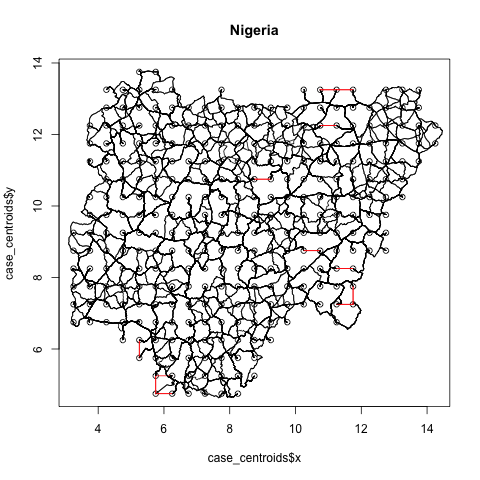
\includegraphics[width=\textwidth, trim={1cm 1cm 0cm 2cm},clip]{/Users/Tilmanski/Documents/UNI/MPhil/Second Year/Thesis_Git/Build/output/Road_Networks/network_Nigeria.png}
\caption{Nigeria}
\label{fig:nigeria_roads}
\end{subfigure}
\begin{subfigure}[c]{0.43\textwidth}
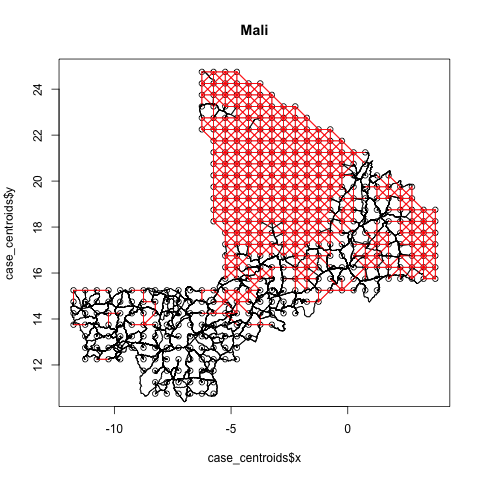
\includegraphics[width=\textwidth, trim={1cm 1cm 0cm 2cm},clip]{/Users/Tilmanski/Documents/UNI/MPhil/Second Year/Thesis_Git/Build/output/Road_Networks/network_Mali.png}
\caption{Mali}
\label{fig:Mali_roads}
\end{subfigure}

\begin{subfigure}[c]{0.43\textwidth}
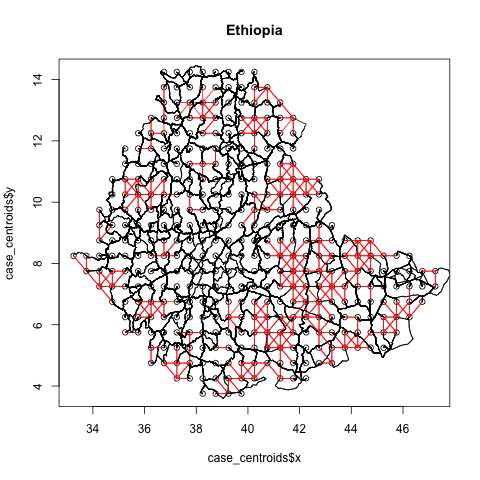
\includegraphics[width=\textwidth, trim={1cm 1cm 0cm 2cm},clip]{/Users/Tilmanski/Documents/UNI/MPhil/Second Year/Thesis_Git/Build/output/Road_Networks/network_Ethiopia.png}
\caption{Ethiopia}
\label{fig:Ethiopia_roads}
\end{subfigure}
\begin{subfigure}[c]{0.43\textwidth}
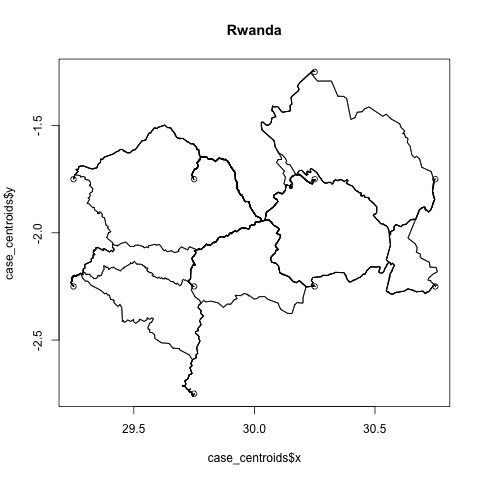
\includegraphics[width=\textwidth, trim={1cm 1cm 0cm 2cm},clip]{/Users/Tilmanski/Documents/UNI/MPhil/Second Year/Thesis_Git/Build/output/Road_Networks/network_Rwanda.png}
\caption{Rwanda}
\label{fig:Rwanda_roads}
\end{subfigure}


\label{fig:roads}
\end{figure}
% End Figure

The OSM routing algorithm is specified for cars and takes into account differential speeds attainable on different types of roads. However, if either start or destination location do not directly fall onto a street, the optimal route jumps to the nearest road and goes from there. To take this into account, I add a walking distance to the travel path. Agents are assumed to walk in straight lines to the nearest street at a fixed speed of 4 km/h. They then take the car and drive the route with average speed as specified by OSM, before they potentially have to walk the last stretch again to their exact centroid destination. For some particularly remote areas, even the nearest street is very far away, such that the car routing provided by OSM is not sensible. To counter these cases, I also calculate for all 90,000 connections the outside option of walking the entire link in a straight line at 4 km/h. I then identify cases in which walking directly is actually faster than using OSM's proposed route (plus the travel to and from roads). In these cases, I replace OSM's route with the walking distance and (constant 4 km/h) speed. Figure \eqref{fig:roads} presents the resulting road networks for two African countries. Figure \eqref{fig:nigeria_roads} displays every optimal route for Nigeria, which appears overall fairly well connected. Commuters mostly seem to be able to drive relatively direct routes between locations, even though cases with substantial detours are also evident at second glance. Connections in which walking were the preferred alternative are displayed in red and fairly rare in Nigeria. Figure \eqref{fig:Mali_roads} presents the case of Mali, which paints a different picture: for many connections through the Sahara desert in the North-East of the country, walking straight lines in the sand is actually the fastest way to get from A to B. Ethiopia in Figure \eqref{fig:Ethiopia_roads} displays only a few trails connecting the country's East to the West. Small Rwanda in Figure \eqref{fig:Rwanda_roads} zooms in on the actual roads taken and displays the intricacies of the optimal routing provided by OSM.

Relying on the open source community of OSM does come with some drawbacks. Most importantly, data on the position and quality of roads is user-generated and hence subject to reporting bias. Intuitively, richer areas may appear to be equipped with more roads if local residents have the time and necessary access to a computer to enter their neighbourhoods into the database. As soon as inference is conducted on the relationship between streets and any covariate of development, the resulting estimates will be biased. While this is certainly troubling, I believe this bias to be much more important on finer resolutions than the operating one in this study. Start and destination of the elicited routes are on average more than 55 kilometres apart and travel will hence take place mostly on larger roads and national highways. It is unlikely that these major streets are systematically underreported in OSM, the primary open source routing platform on the Internet, especially compared to the alternative of digitised Michelin maps. Reporting bias will definitely be an issue when trying to find the optimal route \emph{within} a particular small neighbourhood in Accra, but the OSM database should do a fairly good job in finding the optimal route between Accra and Kumasi. It is nevertheless important to keep this potential flaw of the data in mind when conducting inference later on.\footnote{There is a second, less troubling problem with using OSM data. As this study merely pertains to within-country transport networks, I only look at connections between neighbouring locations of the same country. However, in some cases the optimal route between these locations still might go through a neighbouring country. For instance, Senegal is effectively split into two parts by the intersecting country The Gambia. Still, when connecting Senegalese cell centroids just to the north and to the south of The Gambia (which are still less than 60km apart), the route will go over foreign soil. This presents a problem only in later policy recommendations, as political leaders of one country cannot necessarily legislate road improvements abroad. The rest of the analysis is not affected by this issue.}

In some rare cases (less than 0.1 per cent of all connections), the OSM algorithm cannot find any route between two neighbouring centroid locations. This mostly is due to an obvious geographic impossibility to connect two nodes. In Guinea-Bissau, for instance one location lies on the Bolama Islands just off the shore of mainland Guinea-Bissau. Its neighbouring locations are all on the mainland and hence unreachable by car. In other cases, both locations to be connected are in deep jungle or swampy regions. In all these cases, I treat the link as if the two locations were not neighbours in the first place. That implies I even forgo the backup possibility of walking the entire distance, assuming that agents cannot walk between islands or through the densest jungle.

After having collected data on distance and average speed on the optimal route between all neighbouring centroid locations, the next step is to discretise these data in order to have a tractable network representation capable of performing the trade simulations necessary in the remainder of this study.

\subsubsection{Infrastructure matrix $I_{i,k}$}
To gain a conception of how much two given nodes are connected in the transport network, one needs to derive a numeric measure of how much \emph{current} infrastructure lies on the link between locations. In their own empirical analysis, \cite{fajgelbaum_optimal_2017} have data on the average number on lanes of the streets used on a given route, and whether these streets are national or secondary roads. The OSM algorithm does not supply this detailed level of information for Africa. However, I argue that the authors are only proxying for a much more immediate statistic: the average speed with which one can travel on a given road. If two locations are linked by a faster connection, I assume this to be the result of higher infrastructure $I_{i,k}$ on this edge. Obviously there are many factors influencing driving speed other than number of lanes or road classifications. Congestion, altitude differences, or potholes come to mind. However, what the authors are trying to capture is an infrastructure investment vehicle to reduce trade costs. Certainly building more lanes on a given road will reduce trade costs. But it will do so by increasing the speed with which cars can travel on that road. I argue that observing the average speed with which transport can occur between two nodes is a much more immediate measure of how well these nodes are connected. I hence propose
\begin{equation}
  I_{i,k} = \textrm{Average Speed}_{i,k}
\end{equation}

This measure is naturally bound from below at 4 km/h, as walking the air-line distance is always available as a backup. Empirically, average speeds range between 6 km/h (Mauritania, where most of the distances through the desert have to be covered by walking) and 33 km/h (Swaziland). It is now the objective of the policymaker or social planner to reduce trade costs between suitable trading partners by increasing the average speed $I_{i,k}$ with which transport can occur between them.

\subsubsection{Trade cost parameter $\delta_{i,k}^{\tau}$}
Recall from equation \eqref{eq:tau} that iceberg trade costs between nodes $i$ and $k$ are modelled as $\tau_{i,k}^{n} = \delta^{\tau}_{i, k} \frac{(Q_{i,k}^{n})^{\beta}}{I_{i,k}^{\gamma}}$. Following \citeauthor{fajgelbaum_optimal_2017} and ensuring convexity and strong duality, I parameterise $\beta = 1.245$ and $\gamma = 0.5\beta = 0.6225$.

$\delta^{\tau}_{i, k}$ is a scaling parameter. It impacts trade costs regardless of current infrastructure levels and congestion forces and hence allows for variation caused by exogeneous forces like the geography of a given edge. \citeauthor{fajgelbaum_optimal_2017} calibrate is as a linear function of the distance between $i$ and $k$ and in order to match some particular patterns from Spanish trade data. Their calibration is not applicable to the given context. Firstly, it deals with European developed countries which recent evidence suggests face much less stifling trade costs than the African continent \citep[see e.g.][]{Anderson_Tradecosts_2004}. Secondly, their calibration revolves around different measures for economic output $Y_{i}$ and infrastructure investment $I_{i,k}$ and will hence produce arbitrary estimates for $\delta^{\tau}_{i, k}$.

Instead, I make use of a recent contribution by \cite{atkin_whos_2015}. They use barcode-level data on sale prices of identical goods to back out trade costs between regions within both Nigeria and Ethiopia. They show that trade costs are significantly increasing in distance between origin and destination, stifling much of mutually beneficial trade. In comparison to a similar exercise in the US, the authors again provide evidence that trade costs in Africa are exceptionally dependent on distance travelled. Directly taking the average of their two point estimates for Ethiopia and Nigeria, I calculate
\begin{equation}
  \delta^{\tau}_{i,k} =  0.466\times\textrm{ln}(\textrm{Distance}_{i,k})
  \label{eq:delta_tau}
\end{equation}

as the trade cost elasticity to distance travelled.\footnote{\citeauthor{atkin_whos_2015} (Table 2, page 44) estimate this parameter as $0.0374$ for Ethiopia and $0.0558$ for Nigeria. My parameter is the simple average of these two point estimates.} Note that the functional form of \eqref{eq:tau} still implies that the very first good to be shipped over a given link is free of any trade costs, with convex congestion forces coming into play  afterwards. The social planner can now invest into infrastructure along any link to attenuate these forces.

\subsubsection{Infrastructure building cost matrix $\delta_{i,k}^{I}$}
The \emph{Network Building Constraint} \eqref{eq:network_building} binds the social planner's action space when commissioning faster roads. Total cost of infrastructure $\sum_{i}^{}\sum_{k \in N(i)}^{} \delta_{i,k}^{I}I_{i,k}$ is fixed at $K$, which equals the cost of originally building the current network. In this set-up, $\delta_{i,k}^{I}$ denotes the relative constant cost of increasing the average speed on a given link by one. As $K$ is unrelated to the rest of the model it can be normalised to $K=1$ without loss of generality, so that only relative infrastructure building costs matter. This procedure allows for staying agnostic about the actual (dollar-)cost of building roads and only needs to make a stance on which areas are cheaper or more expensive to build on \emph{relative to others}.

$\delta_{i,k}^{I}$ depends on a variety of inputs, like the distance of a road or the underlying terrain. I follow \citeauthor{fajgelbaum_optimal_2017} who in turn make use of a recent study by \cite{collier_cost_2015} which estimates infrastructure building costs in the Developing World. Readily applying their specification, I calculate
\begin{equation}
  \textrm{ln}(\delta^{I}_{i,k,c}) = \delta_{c}^{I} - 0.11 \times \one_{\textrm{Distance}_{i,k,c} > 50km} + 0.12 \times \textrm{ln}(\textrm{Ruggedness}_{i,k,c}) + \textrm{ln}(\textrm{Distance}_{i,k,c})
  \label{eq:delta_I}
\end{equation}

as the constant cost of increasing infrastructure $I_{i,k}$ on the link between $i$ and $k$ in country $c$. $\textrm{Distance}_{i,k,c}$ denotes the road distance travelled between nodes and enters positively, implying that longer roads are costlier to develop as every single road kilometre will have to be improved. Moreover, the building cost per kilometre falls discretely when the distance surpasses 50 kilometres, as embodied by the indicator $\one_{\textrm{Distance}_{i,k,c} > 50km}$. Note that every route in my sample is longer than 50 kilometres and the corresponding dummy term is hence always equal to 1. $\textrm{Ruggedness}_{i,k,c}$ denotes the average ruggedness between grid cells $i$ and $k$ and enters positively, highlighting the additional expenses accompanied with building on uneven terrain. $\delta_{c}^{I}$ is a country-specific scaling parameter. Its main purpose it to ensure that equation \eqref{eq:network_building} is satisfied with $K=1$. I hence appraise the infrastructure network $I_{i,k}$ of all countries and then flexibly alter $\delta_{0}^{I}$ for each nation individually in order to comply with equation \eqref{eq:network_building}.

It is worth noting that $\textrm{Distance}_{i,k,c}$ denotes the distance travelled along the fastest route as described in section \ref{sec:road_data}, \emph{not} the air-line distance between origin and destination centroid. This is significant in the sense that distance is treated as a primitive of the model and not endogeneously subject to the optimisation exercise. If under the current network two nodes are only connected via an extensive detour, the distance variable as reported by Open Street Maps will be very large. The social planner is now merely equipped with the capacity to improve the infrastructure on the given route, but cannot devise an entirely new road shortcutting the detour. This restriction might very well be reasonable in certain situations. Some nodes might be only connected by a rather circuitous route because of a major geographical obstacle, mountains or swamps, between them. My conception of infrastructure investment ensures that no improbable road through a mountain is devised, but rather the path around the mountain is improved. On the other hand, my model might forgo obvious welfare-improving infrastructure projects based on entirely new roads. In the abstract formalism of the model, this distinction does not make that much of a difference. It can afford to stay agnostic about whether trade costs are decreased by a new shortcut or by road improvements on the old connection. When using the predictions of the model to  inform actual transport policy, however, one has to bear in mind that entirely new roads might at times succeed in connecting regions at even lower costs than the improvements prescribed by my simulation.

\subsection{Heterogeneous goods}
To build incentives for trade, I introduce $N=2$ different goods: an agricultural and an urban good. Since economic output is proxied by night luminosity, I cannot observe the distribution of different goods in a given grid cell, but only their total production. This leads to the total specialisation assumption outlined above in which urban grid cells are solely producing the urban good, while all other grid cells are producing nothing but the agricultural good.

To classify grid cells as urban or rural I use an iterative procedure, which seeks to match each country's 2016 urbanisation rate as reported by \cite{the_world_bank_world_2017}. I start by assuming every location is a city and then gradually proceed to re-classify the least densely populated locations, until the ratio of people living in urban areas to total population equals that of the World Development Indicators.\footnote{For three countries, the WDI do not report urbanisation rates. In these cases, I match the overall urbanisation rate for the entire African continent of 42 per cent as reported by \cite{lall_africas_2017}.} With this procedure, seven per cent of grid cells are classified as urban. These cells inhabit 40 per cent of the continent's population, matching recent figures from \cite{lall_africas_2017} fairly well.

As discussed above, the model stays agnostic about how grid cells produce their luminosity output. This is in contrast to \citeauthor{fajgelbaum_optimal_2017} who allow for endogenous labor allocation across locations and goods and hence need to take a stance on functional forms of total factor productivity and output. The only assumption my model makes is that cells can ever only produce one of the two varieties and their productivity in the respective other variety is zero. I also avoid having to divide total lights by total population in order to obtain TFP, a procedure which has occasionally been used \citep[see e.g.][]{DeLuca_Ethnicfavoritismaxiom_2018}, even though the literature has recently moved towards consensus of warning against it \citep{michalopoulos_spatial_2018}.

\begin{figure}[t]
\centering
\caption{Discretised Networks for different countries}

\begin{subfigure}[c]{0.45\textwidth}
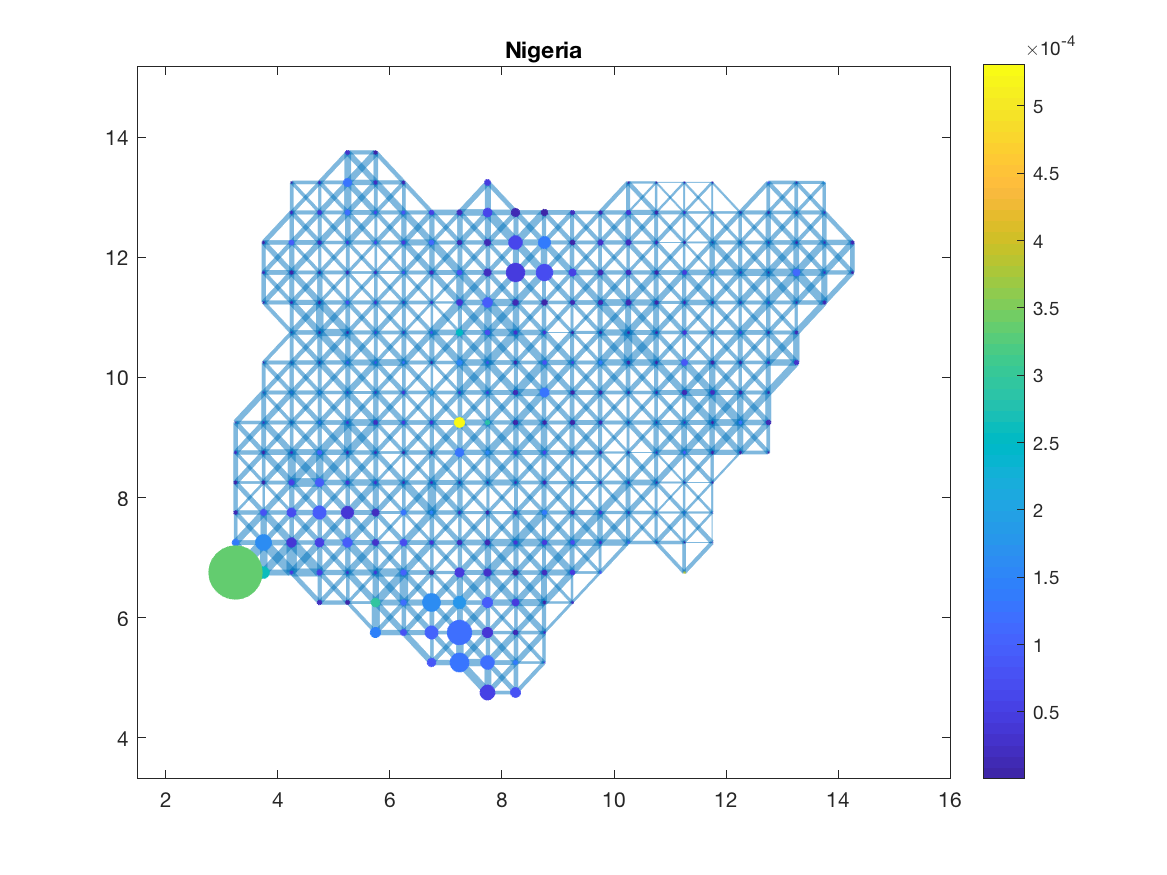
\includegraphics[width=\textwidth, trim={1.6cm 0cm 1.5cm 0cm},clip]{/Users/Tilmanski/Documents/UNI/MPhil/Second Year/Thesis_Git/Build/output/Matlab_graphs/initial_infrastructure/Nigeria_graph.png}
\caption{Nigeria}
\label{fig:nigeria_mat}
\end{subfigure}
\begin{subfigure}[c]{0.45\textwidth}
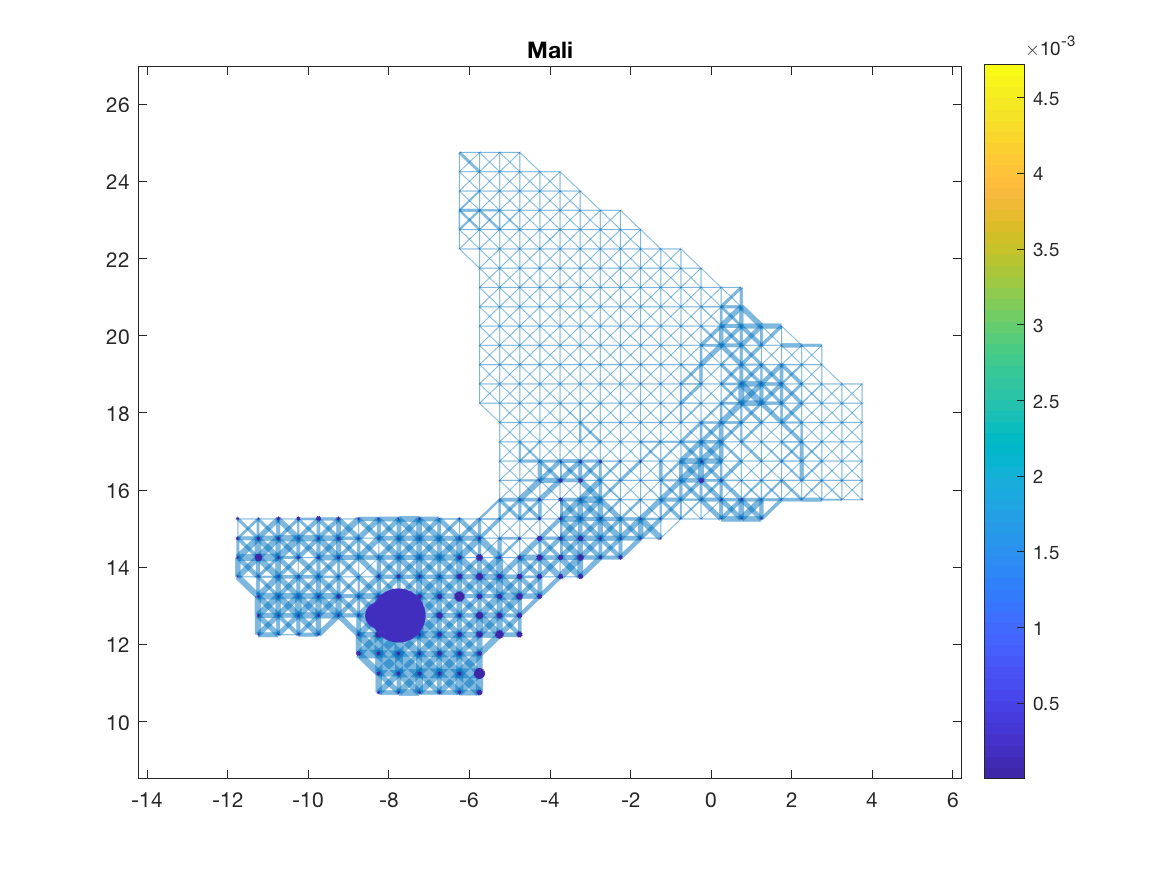
\includegraphics[width=\textwidth, trim={1.6cm 0cm 1.5cm 0cm},clip]{/Users/Tilmanski/Documents/UNI/MPhil/Second Year/Thesis_Git/Build/output/Matlab_graphs/initial_infrastructure/Mali_graph.png}
\caption{Mali}
\label{fig:Mali_mat}
\end{subfigure}

\begin{subfigure}[c]{0.45\textwidth}
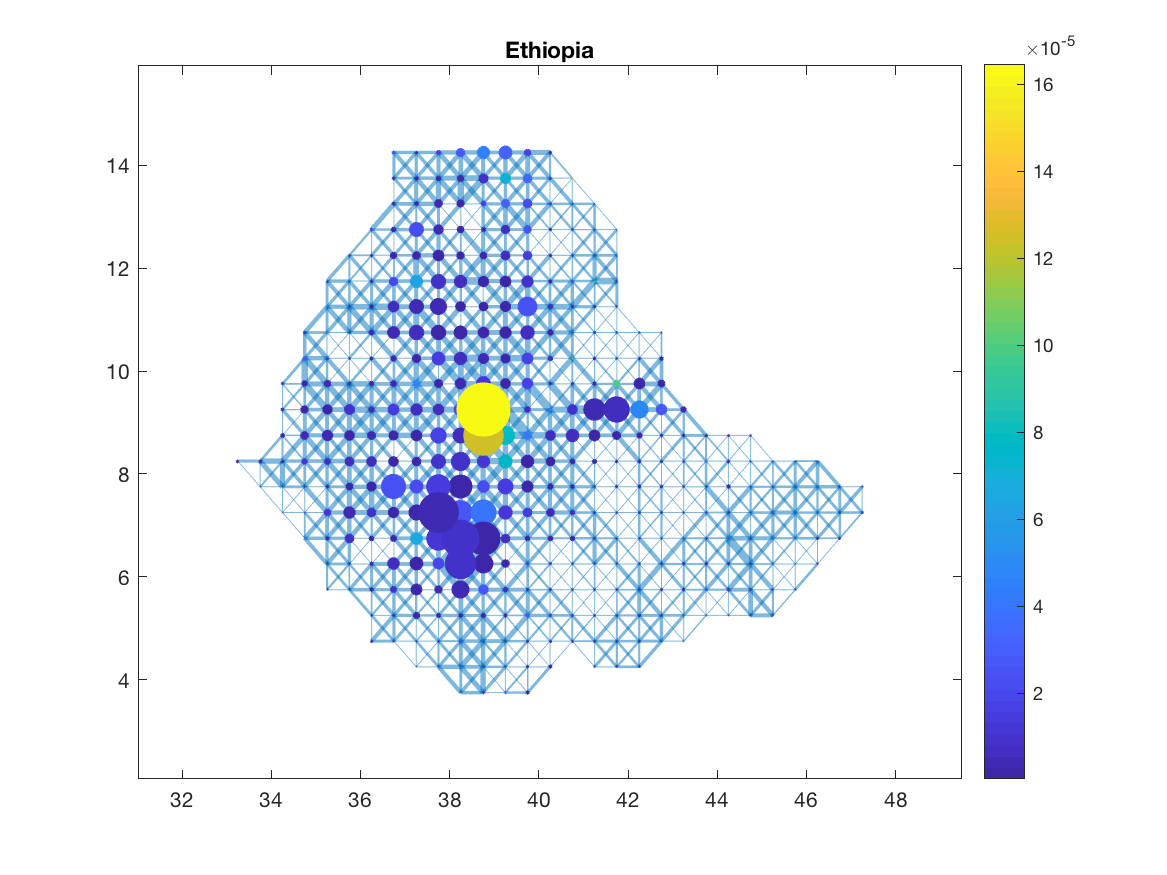
\includegraphics[width=\textwidth, trim={1.6cm 0cm 1.5cm 0cm},clip]{/Users/Tilmanski/Documents/UNI/MPhil/Second Year/Thesis_Git/Build/output/Matlab_graphs/initial_infrastructure/Ethiopia_graph.png}
\caption{Ethiopia}
\label{fig:Ethiopia_mat}
\end{subfigure}
\begin{subfigure}[c]{0.45\textwidth}
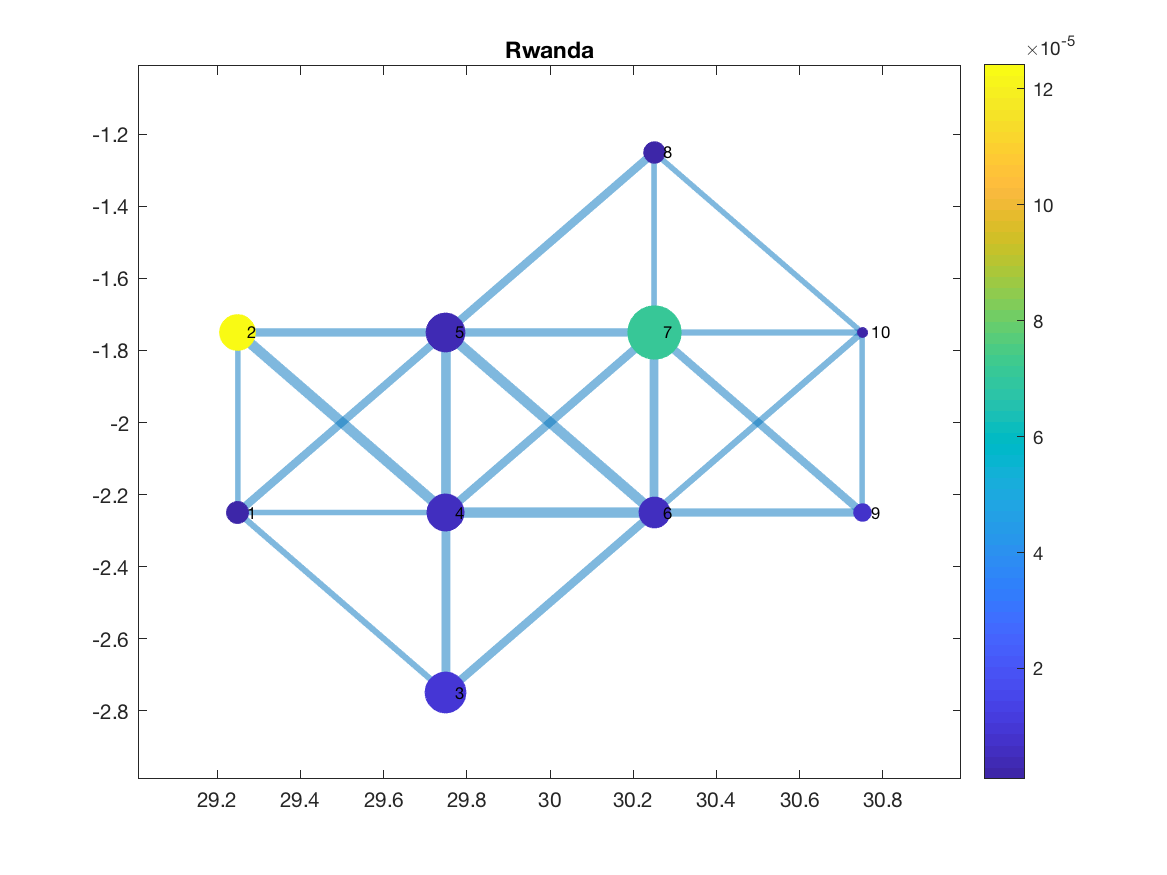
\includegraphics[width=\textwidth, trim={1.6cm 0cm 1.5cm 0cm},clip]{/Users/Tilmanski/Documents/UNI/MPhil/Second Year/Thesis_Git/Build/output/Matlab_graphs/initial_infrastructure/Rwanda_graph.png}
\caption{Rwanda}
\label{fig:Rwanda_mat}
\end{subfigure}
\label{fig:matlab_networks}
\end{figure}

\subsection{Simulation}

After these steps, a discretised network representation now exists for every African country. Nodes in the network are the spaced centroid locations of each grid cell. They combine the characteristics of the entire grid cell (population, output, etc.) in one point. Edges in the network are road connections between centroids. Each edge carries a number of characteristics (average speed, trade costs, and infrastructure building costs). Figure \eqref{fig:matlab_networks} presents this discretised network specification for the four countries from above. Nodes are printed larger proportional to their population. A node's colour scale reflects night light intensity per capita (a statistic which is only calculated for illustrative purposes). Edges are drawn thicker proportional to the initial infrastructure investment (i.e. average attainable speed).

For each country, I proceed to conduct two simulation exercises. In the first, infrastructure $I_{i,k}$ is treated as fixed. This is to obtain a baseline estimate of the spatial variation of welfare in each country. Locations are still allowed to trade with each other, but only over the exogeneous current road network. Formally, this corresponds to solving a slightly truncated version of the social planner exercise from above, where $I_{i,k}$ is simply dropped from the planner's set of control variables.\footnote{Recall that the optimal network allocation exercise nests the problem of solving for optimal trade flows. Hence, every other aspect of the model remains unaffected by fixing $I_{i,k}$. Note that this makes the \emph{Network Building Constraint} \eqref{eq:network_building} non-binding. The same outcome could be achieved by introducing an additional constraint $I_{i,k} = I_{i,k}^{\textrm{empirical}}$, however at higher computational requirements.} By construction, the resulting solution will have two properties. Firstly, total output over the entire country will remain untouched. Inputs are not defined and hence do not shift to more productive regions. Indeed, any welfare gains will be attained solely by shipping the right mix of goods to the right regions. Secondly, labor immobility will leave welfare differences between regions as agents cannot simply move to more privileged cells. The social planner would like to overcome these differences, but is confronted with trade costs which might leave certain remote areas much worse off than well-connected ones.

Following this static exercise, I proceed to the main task of endogeneising the infrastructure matrix $I_{i,k}$. With the \emph{Network Building Constraint} binding total infrastructure investment at the level of the current road network, the social planner is now free to reshuffle roads within the country in order to improve connections as she chooses. If she wants to improve the connection between two given locations, she will have to take away infrastructure from somewhere else in the country. Intuitively, this reallocation exercise does not seek to identify where to place the optimal next investment, but rather represents an utterly fictitious scenario in which every road can be lifted from the ground, reshuffled, and eventually located someplace else.\footnote{Note that equation \eqref{eq:network_building} only fixes $\sum_{i}^{}\sum_{k \in N(i)}^{} \delta_{i,k}^{I}I_{i,k} = K$. Hence, not the overall sum of infrastructure is fixed, but more precisely the overall cost of infrastructure. This still allows the social planner to take away one unit of infrastructure on a very expensive (high $\delta_{i,k}^{I}$) link and exchange it for much more than one unit on a cheaper (low $\delta_{i,k}^{I}$) link.} The procedure does not measure how many roads a country has, but rather how well they are placed. It does not look at whether the entire country is full of speedy roads, but rather whether those roads connect the right locations.

I conduct the reallocation scenario for every African country. Five small countries (Cape Verde, Comoros, The Gambia, Mauritius, and Reunion) are too small to form a sensible network as they only show up as a single location in the dataset and are henceforth no longer considered. Computation times are greatly diminished when exploiting the strong convexity of the optimisation setting and solving the dual problem as sketched in the technical appendix of \cite{fajgelbaum_optimal_2017}. Optimisations are performed via Matlab's \texttt{fmincon} command. When conducting the simulations, I bind the social planner's set of permissible roads from below, at 4 km/h (such that $I_{i,k} \geq 4$ $ \forall \textrm{ } i,k$). This is motivated by the assumption at the beginning that walking straight lines at this speed is conceived as an outside option and always available to any commuter. The social planner should not be able to force commuters to travel slower than walking, in order to build a faster road elsewhere.\footnote{Contrarily, I do not explicitly restrict possible investments from above (at least not in addition to the sum-restriction imposed by Equation \eqref{eq:network_building}), as this could violate the strong convexity of the problem. Not bounding the problem in principle allows the social planner to combine every available infrastructure from all over the country into one supersonic speed highway on one particular node. However, the model is calibrated in a way that makes this very unattractive to the planner anyway. After simulating reallocation in every African country, less than 0.8\% of all built roads were suggested to be over 260 km/h. Still, one outlier of 2007 km/h (in Egypt) and one of 1755 km/h (in South Africa) remain.}

\begin{figure}[!h]
\centering
\caption{Reallocation Scenario for different countries}

\begin{subfigure}[c]{0.45\textwidth}
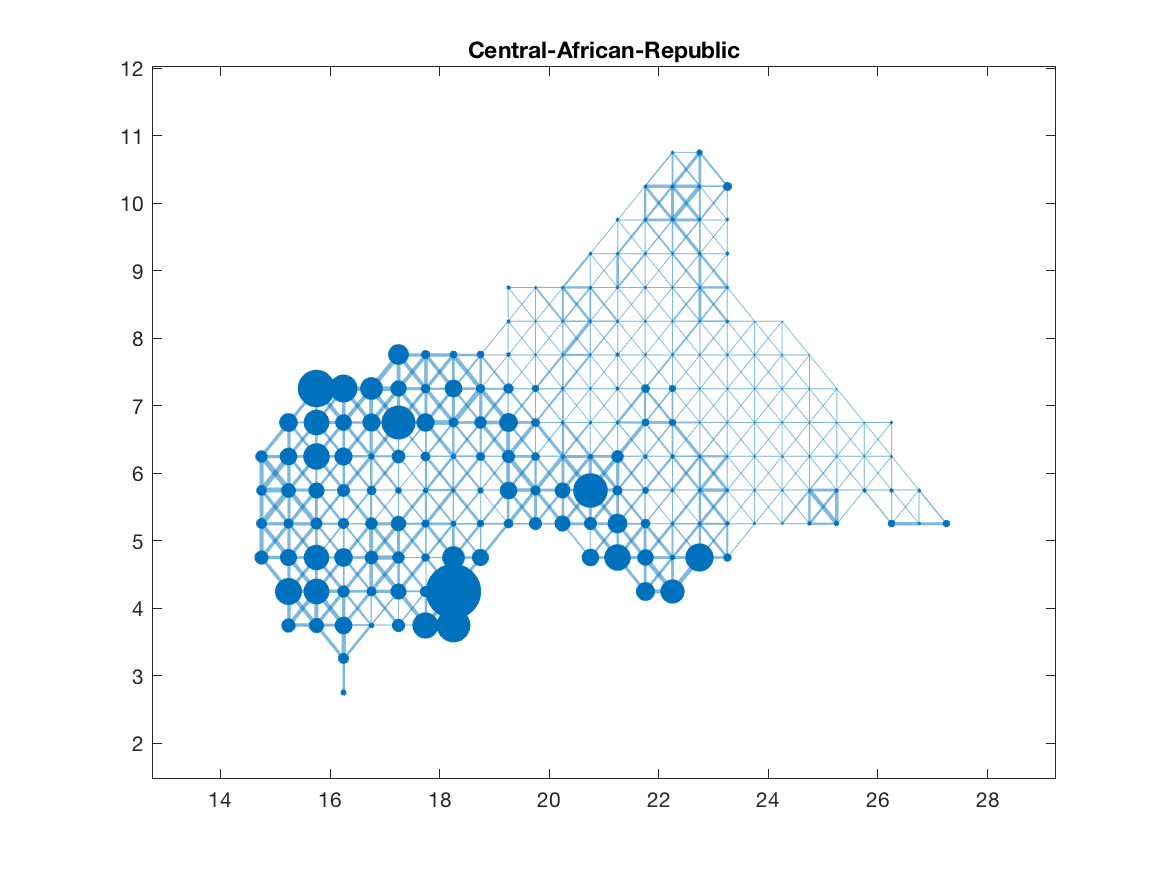
\includegraphics[width=\textwidth, trim={2cm 1cm 1.5cm 0cm},clip]{/Users/Tilmanski/Documents/UNI/MPhil/Second Year/Thesis_Git/Build/output/Matlab_graphs/Nicer_graphs/Central-African-Republic_stat.png}
\caption{Central African Republic, pre reallocation}
\label{fig:cae_pre}
\end{subfigure}
\begin{subfigure}[c]{0.45\textwidth}
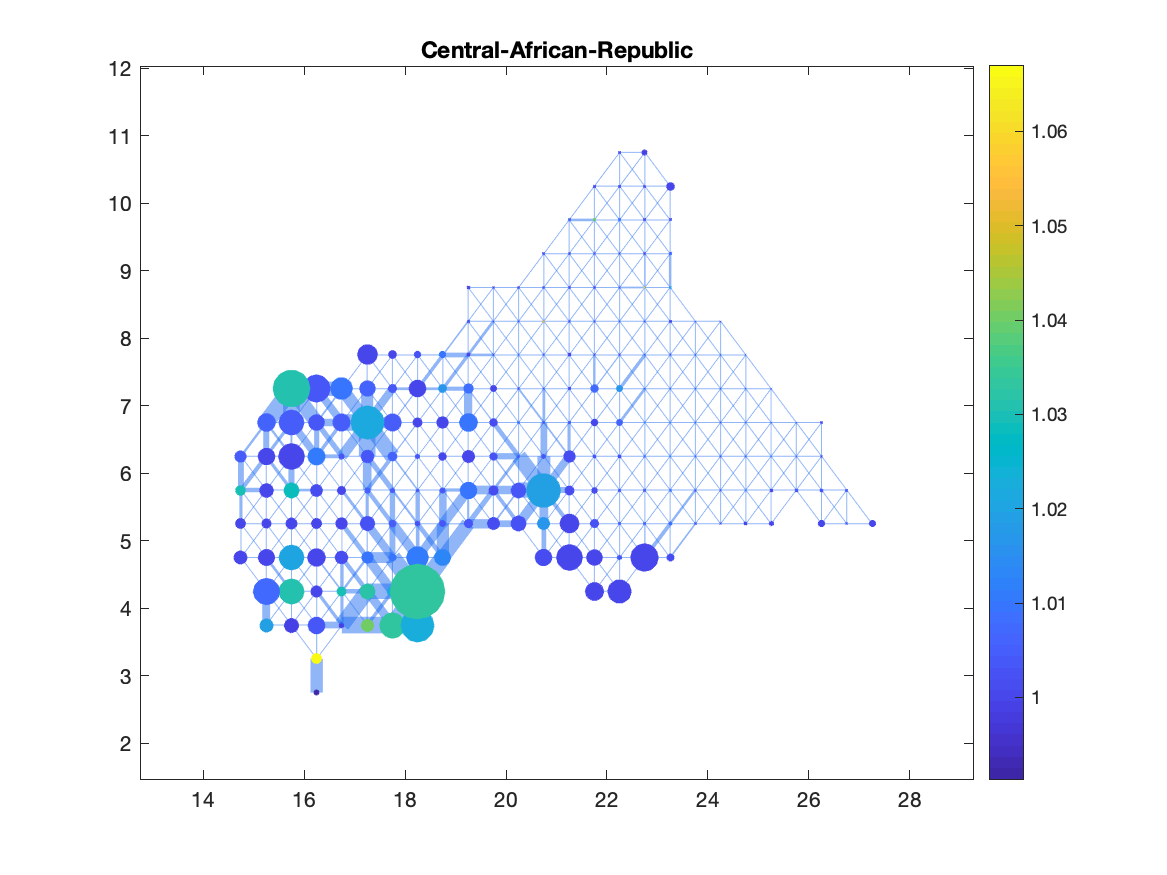
\includegraphics[width=\textwidth, trim={2cm 1cm 1.5cm 0cm},clip]{/Users/Tilmanski/Documents/UNI/MPhil/Second Year/Thesis_Git/Build/output/Matlab_graphs/Nicer_graphs/Central-African-Republic_opt.png}
\caption{Central African Republic, post reallocation}
\label{fig:cae_post}
\end{subfigure}

\begin{subfigure}[c]{0.45\textwidth}
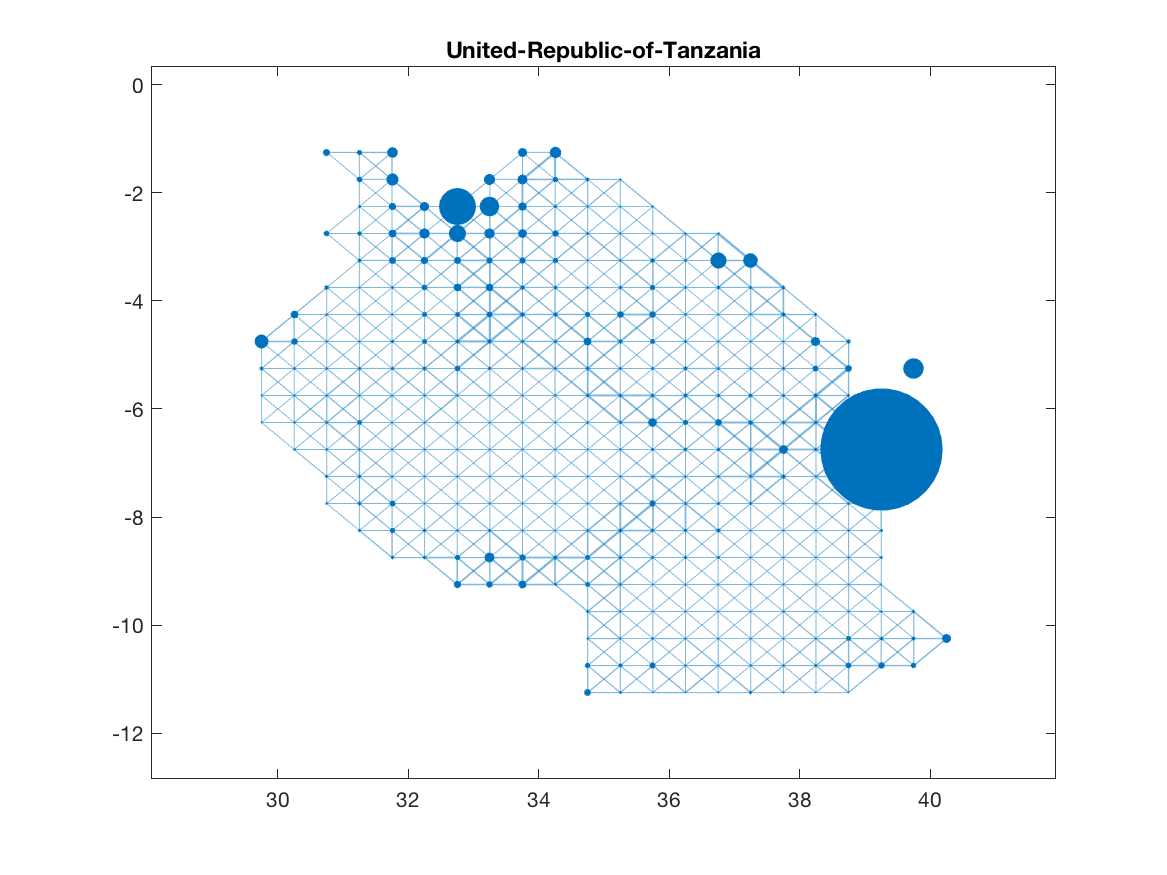
\includegraphics[width=\textwidth, trim={2cm 1cm 1.5cm 0cm},clip]{/Users/Tilmanski/Documents/UNI/MPhil/Second Year/Thesis_Git/Build/output/Matlab_graphs/Nicer_graphs/United-Republic-of-Tanzania_stat.png}
\caption{Tanzania, pre reallocation}
\label{fig:tanzania_pre}
\end{subfigure}
\begin{subfigure}[c]{0.45\textwidth}
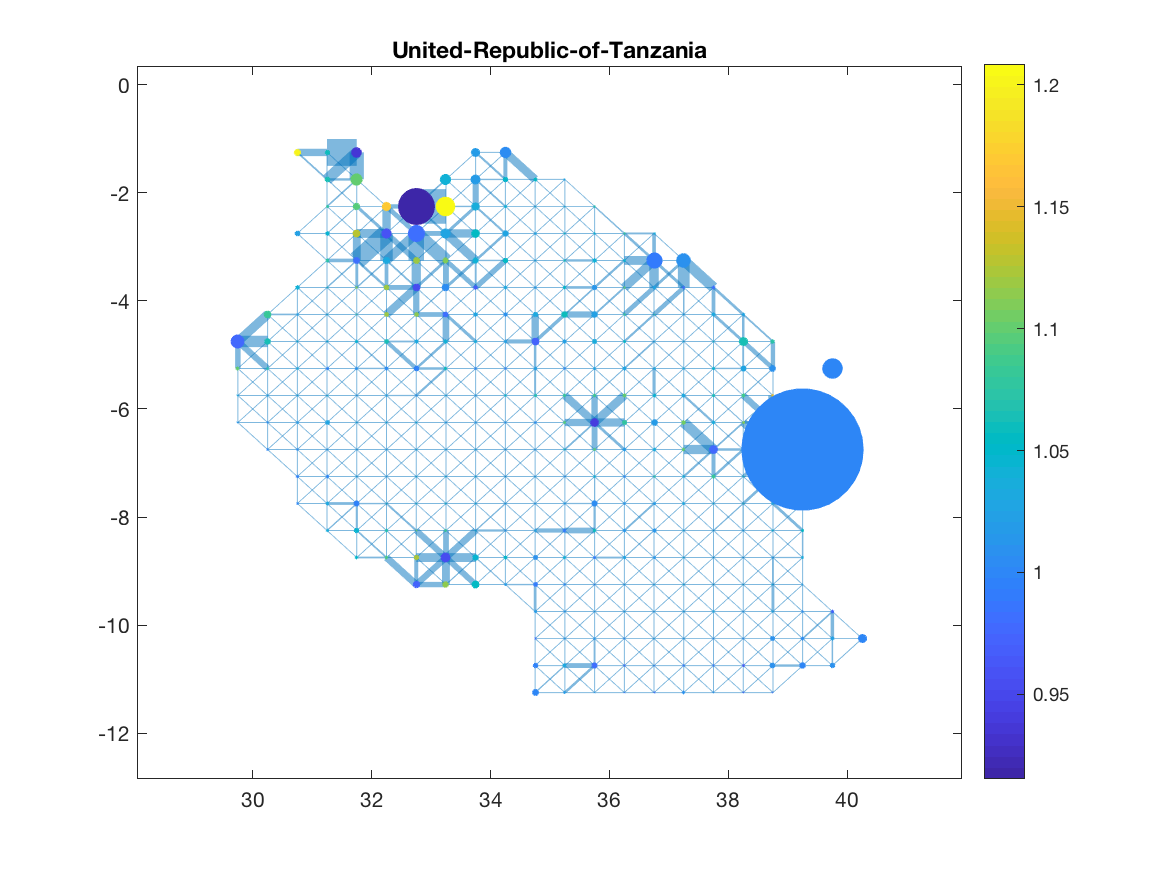
\includegraphics[width=\textwidth, trim={2cm 1cm 1.5cm 0cm},clip]{/Users/Tilmanski/Documents/UNI/MPhil/Second Year/Thesis_Git/Build/output/Matlab_graphs/Nicer_graphs/United-Republic-of-Tanzania_opt.png}
\caption{Tanzania, post reallocation}
\label{fig:tanzania_post}
\end{subfigure}

\begin{subfigure}[c]{0.45\textwidth}
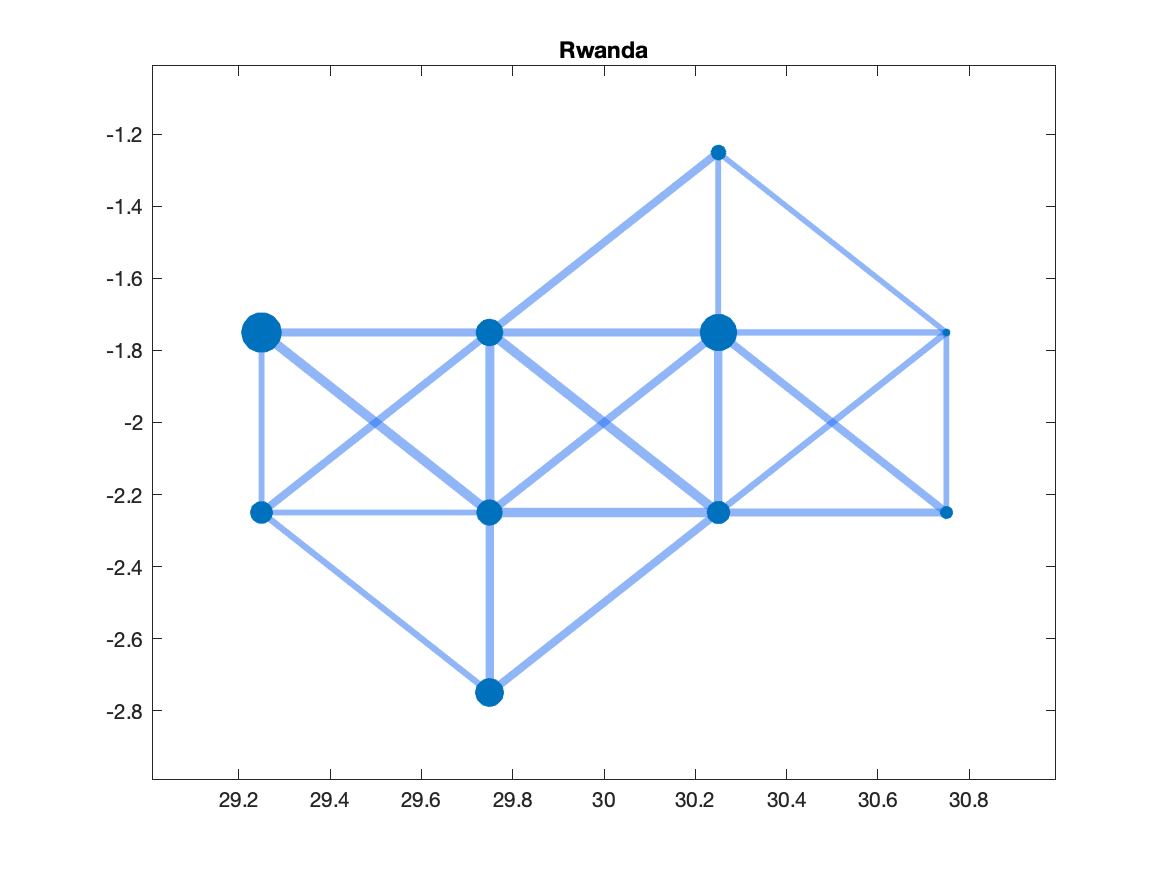
\includegraphics[width=\textwidth, trim={2cm 0cm 1.5cm 0cm},clip]{/Users/Tilmanski/Documents/UNI/MPhil/Second Year/Thesis_Git/Build/output/Matlab_graphs/Nicer_graphs/Rwanda_stat.png}
\caption{Rwanda, pre reallocation}
\label{fig:rwanda_pre}
\end{subfigure}
\begin{subfigure}[c]{0.45\textwidth}
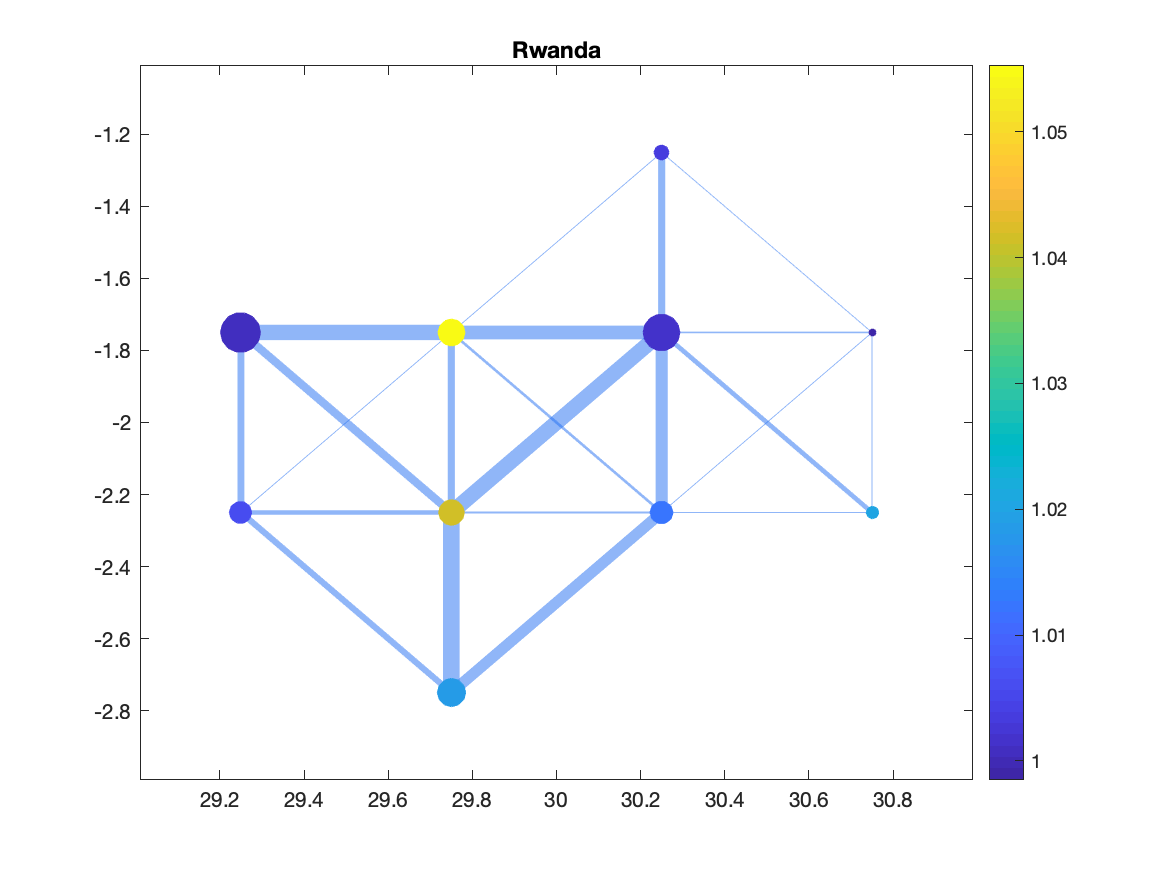
\includegraphics[width=\textwidth, trim={2cm 0cm 1.5cm 0cm},clip]{/Users/Tilmanski/Documents/UNI/MPhil/Second Year/Thesis_Git/Build/output/Matlab_graphs/Nicer_graphs/Rwanda_opt.png}
\caption{Rwanda, post reallocation}
\label{fig:rwanda_post}
\end{subfigure}

\label{fig:Reallocations}
\end{figure}

Figure \eqref{fig:Reallocations} visualises this reallocation exercise for several countries. Subfigure \eqref{fig:cae_pre} displays the discretised network representation of the Central African Republic, comparable to figures \eqref{fig:nigeria_mat} -- \eqref{fig:Rwanda_mat}. The edges to this network are printed almost evenly thick, implying that infrastructure is fairly evenly distributed across the country. Subfigure \eqref{fig:cae_post} then displays the country after the network reshuffling exercise. Three patterns stand out. First, the social planner sees a clear need to connect the populous areas in the South West of the country with each other. Some southern nodes are granted extensive, almost highway-like connections to their immediate neighbours. For that, the social planner is willing to salvage some of the apparently unnecessary infrastructure in the middle or north of the country. Second, there still seems to be a benefit from having a few trails connecting the South West with the North East. Some clear North-South and East-West trails spanning multiple regions emerge. Thirdly, Figure \eqref{fig:cae_post} prints nodes in a colour scale corresponding to individual welfare gains and losses for each location. As can be seen from first-glance, most southern regions stand to gain between five to ten per cent of total welfare from this scenario. Hardly any nodes seem to lose welfare, even though on second glance a few instances become apparent.

Tanzania in Figures \eqref{fig:tanzania_pre} -- \eqref{fig:tanzania_post} displays a more decentralised optimal network solution. The reallocation scenario results in the main urban areas being better connected to their immediate surroundings, but no clear overarching network seems to emerge. There also does not appear to be any necessity to connect hinterland regions with the primal city Dar es Salaam in the West. Indeed, the largest city slightly loses welfare with the reallocation at the expense of multiple smaller population centres in the North.\footnote{On a sidenote, Tanzania also illustrates an interesting case where a tiny fraction of the country is fully detached from the rest of the network. Just north of Dar es Sallam, the island of Zanzibar constitutes a one-node subnetwork of its own. Not surprisingly, it remains completely unaffected by the reshuffling of roads on the mainland. Instances like these are relatively common in the dataset.} Small Rwanda in Figures \eqref{fig:rwanda_pre} -- \eqref{fig:rwanda_post} helps illustrating some of the forces at hand in a less crowded graph. Starting from a fairly evenly distributed transport network, the reallocation dynamics lead to much more variation in infrastructure provision. Some links are deemed superfluous and hence reduced to the smallest admissible level, while others are scaled multiple times their starting infrastructure level. Furthermore, high welfare gains are reported by direct neighbours of big production centres and urban grid cells. These are unassuming grid cells with average population or output levels, merely equipped with the geographical blessing of being close to a bigger neighbour. This leads to the conclusion that while better infrastructure combats the welfare costs of geographical distance, proximity to hubs still matters. Even an optimally designed transport network is ultimately not able to overcome the \emph{curse of distance}.\footnote{A term coined by \cite{Boulhol_Havedevelopedcountries_2010}.}

After successfully reshuffling a country's transport network, overall welfare will necessarily (weakly) increase. It is the social planner's objective to maximise overall welfare, and since the original network composition is always still available, the entire country cannot on aggregate be worse off than before. Note again that overall production (light output) will be unaffected by the entire exercise. Welfare gains are solely caused by enabling mutual benefits from trade through connecting the right locations. Nevertheless, welfare gains are substantial. The Central African Republic of Figure \eqref{fig:Reallocations}, for instance, stands to gain 1.84\% of overall welfare just by reshuffling its roads. Since this welfare gain is rather hard to materialise, I prefer thinking of it as a measure of network inefficiency. The higher the hypothetical gains from merely reshuffling existing roads, the more haphazard the existing allocation of roads, and hence the more inefficient the current transport network.

\begin{figure}
\centering
\caption{African countries by network inefficiency}
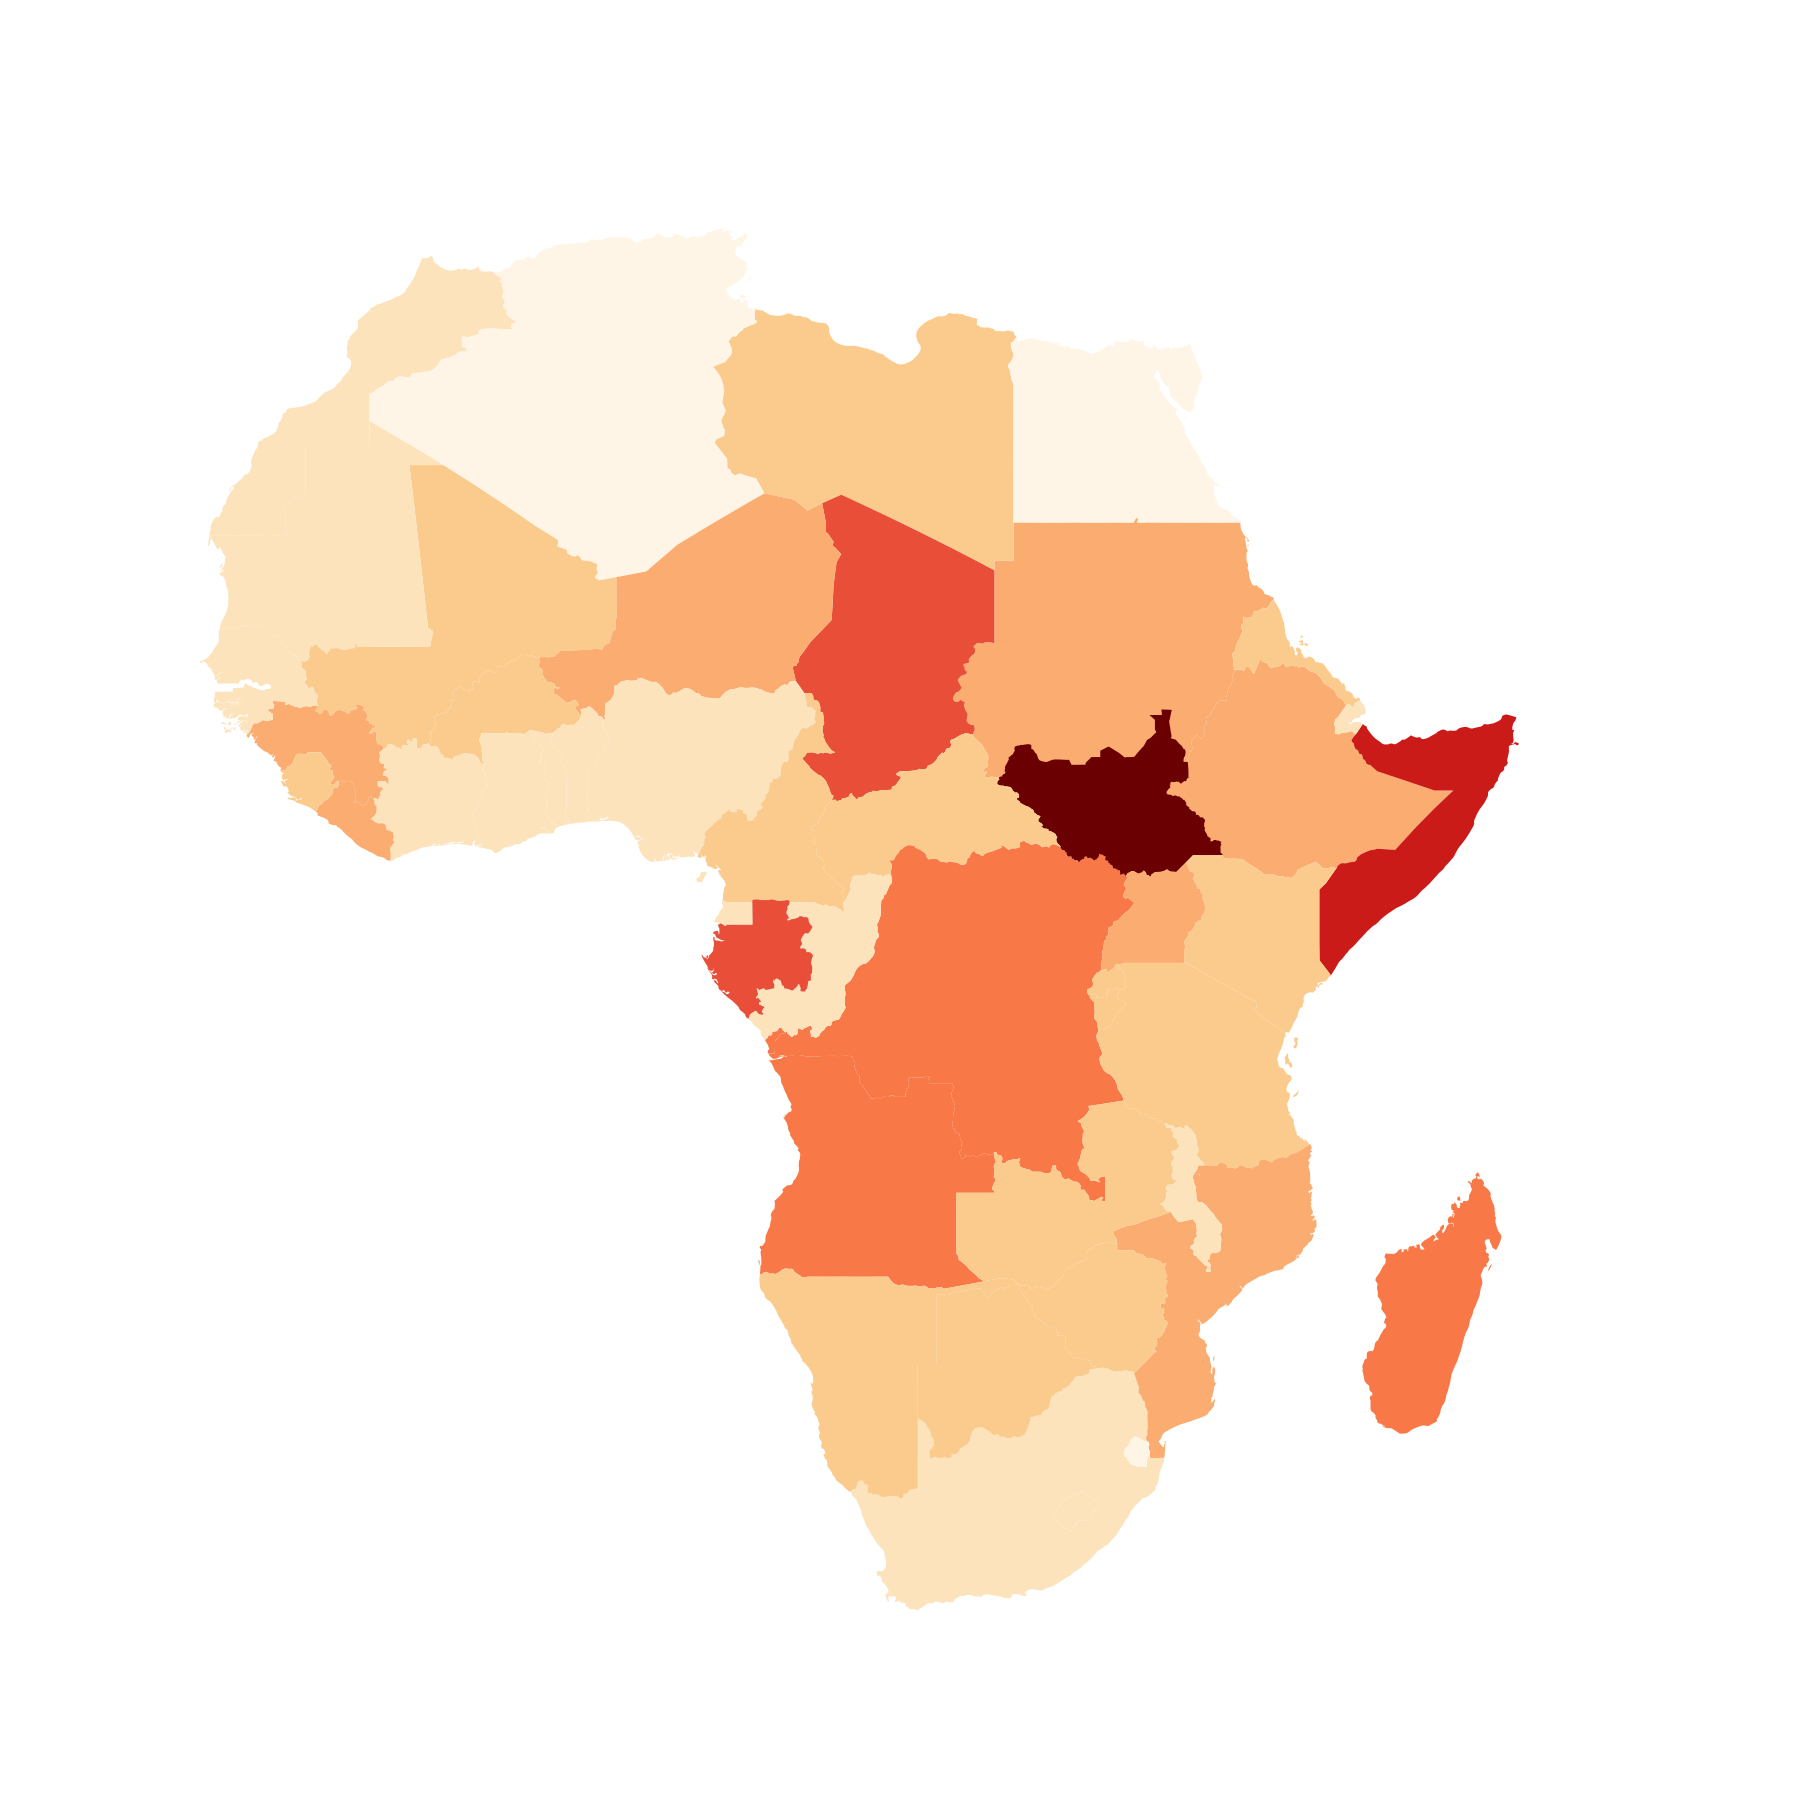
\includegraphics[width=0.6\textwidth]{/Users/Tilmanski/Documents/UNI/MPhil/Second Year/Thesis_Git/Analysis/output/zeta_heatmaps/African_countries_zeta.png}

\label{fig:countries_by_welfare_gain}
\end{figure}

Figure \eqref{fig:countries_by_welfare_gain} displays all African countries and their measure of network inefficiency. The closer the forgone welfare gain to zero (the lighter the country's colour), the more efficient the current allocation of roads. The Central African Republic's measure of 1.84\% makes the country look rather good in comparison. Some (mostly more developed) countries like South Africa (0.47\%) or Tunisia (0.24\%) perform even better. Many countries are leaving much more on the table like Somalia (4.76\%) or Chad (4.28\%). No African country, however, has a more ill advised road network than South Sudan (6.66\%). This might not come as a surprise, as the world's youngest country has largely inherited a road network that was not conceived to sustain an independent nation, but connect it to its former capital up north. On a simple cross-country level, more inefficient networks are significantly correlated with more corruption ($p < 0.01$), less property rights ($p < 0.01$) and less 2010 log GDP ($p=0.07$). Note that these are merely descriptive correlations which are far from implying any form of causation.\footnote{Data from \cite{the_world_bank_world_2017}. For corruption and property rights, data is only available for 35 countries and correlations are hence performed on this truncated sample.}

While each country only stands to gain overall welfare from this reallocation procedure, individual locations might very well lose in the process. Intuitively, some regions might be equipped with far too many good roads such that the social planner takes these roads away to use someplace else. Comparing each grid cell's welfare before and after the major reshuffling can help identify regions which are currently over or under-provided for. More formally, I define

\begin{equation}
  \zeta_{i} = \frac{\textrm{Welfare under the optimal Infrastructure}_{i}}{\textrm{Welfare under the current Infrastructure}_{i}}
\end{equation}

% Figure
\begin{figure}
\centering
\caption{Spatial Distribution of $\zeta_{i}$ for sample countries}

\begin{subfigure}[c]{0.32\textwidth}
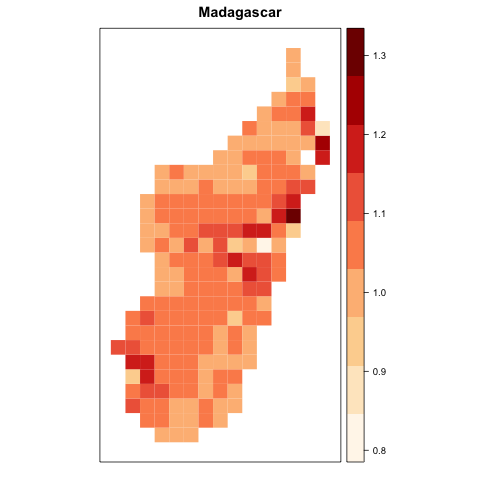
\includegraphics[width=\textwidth]{/Users/Tilmanski/Documents/UNI/MPhil/Second Year/Thesis_Git/Analysis/output/zeta_heatmaps/Madagascar_zeta.png}
\caption{Madagascar}
\label{fig:Madagascar_zeta}
\end{subfigure}
\begin{subfigure}[c]{0.32\textwidth}
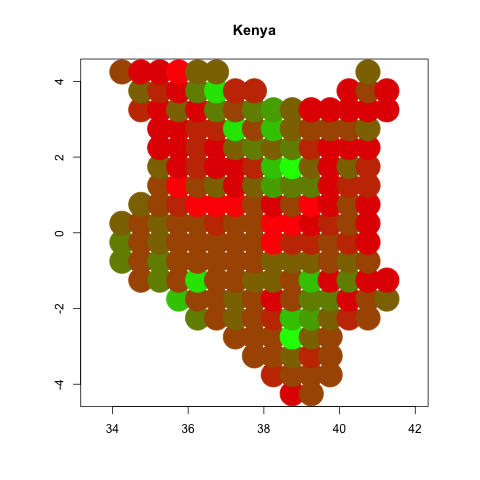
\includegraphics[width=\textwidth]{/Users/Tilmanski/Documents/UNI/MPhil/Second Year/Thesis_Git/Analysis/output/zeta_heatmaps/Kenya_zeta.png}
\caption{Kenya}
\label{fig:Kenya_zeta}
\end{subfigure}
\begin{subfigure}[c]{0.32\textwidth}
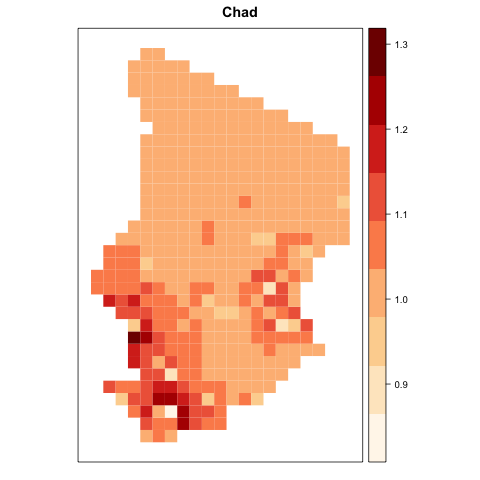
\includegraphics[width=\textwidth]{/Users/Tilmanski/Documents/UNI/MPhil/Second Year/Thesis_Git/Analysis/output/zeta_heatmaps/Chad_zeta.png}
\caption{Chad}
\label{fig:Chad_zeta}
\end{subfigure}
\label{fig:zeta_countries}
\end{figure}
% End Figure

as the \emph{Infrastructure Gap} for each grid cell $i$. Figure \eqref{fig:zeta_countries} displays the spatial distribution of the infrastructure gap $\zeta_{i}$ for Madagascar, Kenya, and Chad. The darker a grid cell's shade, the more it is disadvantaged by the inefficiencies of the current network. The lighter a cell, the more overprovided a region is with infrastructure.

% Figure
\begin{figure}
\centering
\caption{Spatial Distribution of $\zeta_{i}$ for entire sample}
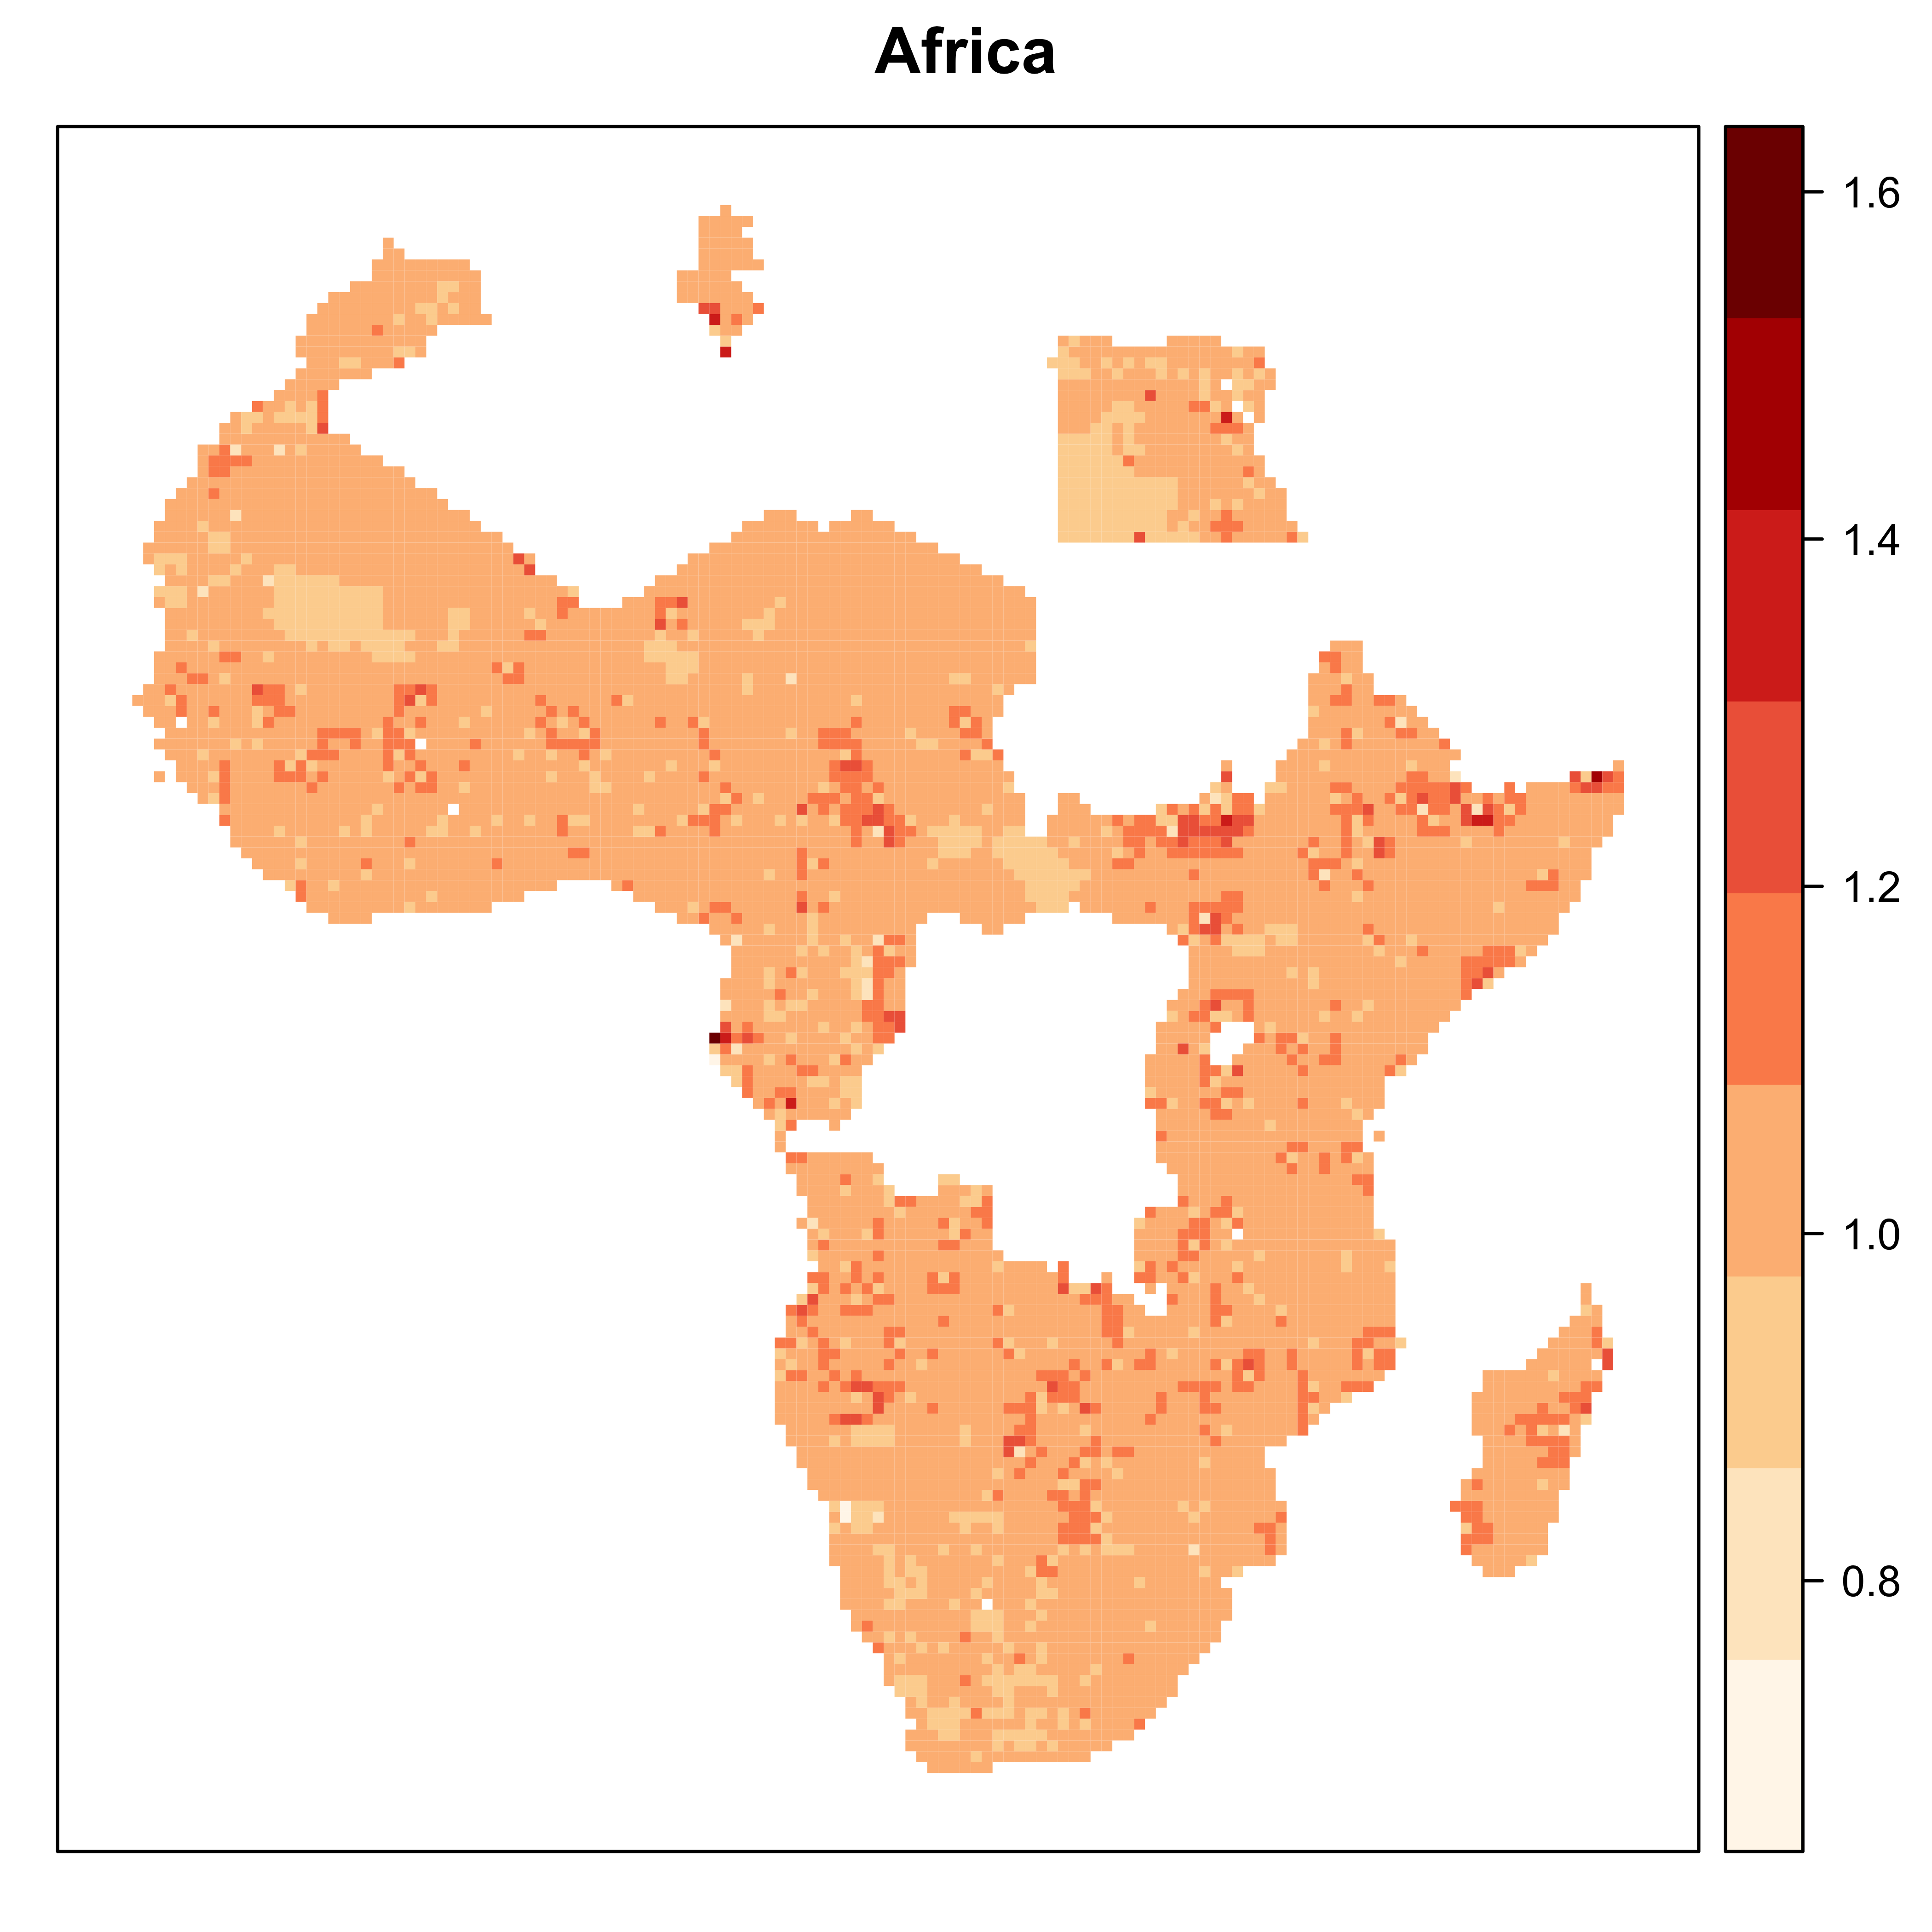
\includegraphics[width=0.65\textwidth,trim={1cm 1cm 1cm 1cm},clip]{/Users/Tilmanski/Documents/UNI/MPhil/Second Year/Thesis_Git/Analysis/output/zeta_heatmaps/African_gridcells_zeta.png}

\label{fig:all_gridcells_by_zeta}
\end{figure}
% End Figure

Figure \eqref{fig:all_gridcells_by_zeta}, lastly, displays the spatial variation of $\zeta_{i}$ over all 10,000+ grid cells of the entire African continent. When interpreting this map, note that grid cells are undergoing the reshuffling scenario solely within their respective country. National borders hence play a role and can at times even clearly be inferred from the printed map. Keeping this in mind, the map reveals substantial spatial variation in the infrastructure gap across the African continent. The luckiest region (in Namibia) stands to loose almost 30\% of total welfare if the fictitious social planner intervened and reshuffled roads away from. On the other hand of the spectrum, the residents of one grid cell in Gabon are missing out on a welfare hike of more than 50\%. Moreover, abandoned regions are clearly displaying spatial correlation with large neighbouring swaths of land collectively missing out on infrastructure improvements in certain countries. This begs the conclusion that countries do not just overlook single grid cells but rather live with vast stretches of disadvantaged regions.

In the following section, I proceed to investigate the patterns behind this heterogeneity of network inefficiency over space.
% End Chapter

\section{Results}



% Figure
\begin{table}[] \centering
  \caption{Colonial Railroads and Infrastructure Gap}
  \label{RailKM_zeta}
  \resizebox{\textwidth}{!}{

  \begin{tabular}{@{\extracolsep{5pt}}lcccccccc}
  \\[-1.8ex]\hline
  \hline \\[-1.8ex]
   & \multicolumn{8}{c}{\textit{Dependent variable:}} \\
  \cline{2-9}
  \\[-1.8ex] & \multicolumn{8}{c}{Infrastructure Gap $\zeta_{i}$} \\
  \\[-1.8ex] & (1) & (2) & (3) & (4) & (5) & (6) & (7) & (8)\\
  \hline \\[-1.8ex]
   KM of Colonial Railroads & $-$0.0002$^{***}$ & $-$0.0001$^{***}$ & $-$0.0002$^{***}$ & $-$0.0002$^{***}$ &  &  &  &  \\
    & (0.0001) & (0.0001) & (0.0001) & (0.0001) &  &  &  &  \\
    & & & & & & & & \\
   KM of Colonial Placebo Railroads &  &  &  &  & 0.00004 & $-$0.0002 & $-$0.0003 & $-$0.0003 \\
    &  &  &  &  & (0.0003) & (0.0003) & (0.0003) & (0.0003) \\
    & & & & & & & & \\
  \hline \\[-1.8ex]
  Country FE &  & Yes & Yes & Yes &  & Yes & Yes & Yes \\
  Geographic controls &  &  & Yes & Yes &  &  & Yes & Yes \\
  Simulation controls &  &  &  & Yes &  &  &  & Yes \\
  Observations & 10,158 & 10,158 & 10,158 & 10,158 & 10,158 & 10,158 & 10,158 & 10,158 \\
  R$^{2}$ & 0.001 & 0.099 & 0.112 & 0.114 & 0.00000 & 0.098 & 0.111 & 0.113 \\
  \hline
  \hline \\[-1.8ex]
  \textit{Note:}  & \multicolumn{8}{r}{$^{*}$p$<$0.1; $^{**}$p$<$0.05; $^{***}$p$<$0.01} \\
  \end{tabular}

}

\justify
\textit{\\ \footnotesize This table displays results of estimation of equation \eqref{eq:regression} on the sample of 0.5x0.5 degree grid cells for the entire African continent (excluding five small countries, see text). Dependent variable is the infrastructure gap for each grid cell. Columns (1)-(4) estimate the effect of colonial infrastructure investments on today's infrastructure gap. Starting with a simple univariate cross-section in (1), column (2) adds 49 country-fixed effects. Column (3) adds geographic controls, consisting of altitude, temperature, average land suitability, malaria prevalence, yearly growing days, average precipitation, the fourth-order polynomial of latitude and longitude, and an indicator of whether the grid cell lies on the border of a country's network. Simulation controls are added in column (4) and are comprised of population, night lights, ruggedness, and a dummy for whether a cell is classified as urban. These are indicators that went into the original infrastructure re-allocation simulation and are hence not orthogonal to $\zeta$. Columns (5)-(8) repeat these calculations with railroads that were planned, but never built (``placebo railroads''). Results are robust to using only the subsample of 33 countries with any colonial infrastructure investment as reported by \cite{jedwab_permanent_2016}, plus South Africa. Heteroskedasticity-robust standard errors are clustered on the 3x3 degree level and are shown in parantheses.}
\end{table}
% End Figure


% Figure
\begin{table}[] \centering
  \caption{General Equilibrium Effects of Colonial Railroads}
  \label{RailBlocks_zeta}
  \resizebox{\textwidth}{!}{


  \begin{tabular}{@{\extracolsep{5pt}}lcccccccc}
  \\[-1.8ex]\hline
  \hline \\[-1.8ex]
   & \multicolumn{8}{c}{\textit{Dependent variable:}} \\
  \cline{2-9}
  \\[-1.8ex] & \multicolumn{8}{c}{Infrastructure Gap $\zeta_{i}$} \\
  \\[-1.8ex] & (1) & (2) & (3) & (4) & (5) & (6) & (7) & (8)\\
  \hline \\[-1.8ex]
   $<10$ KM to Colonial Railroad & $-$0.013$^{***}$ & $-$0.015$^{***}$ & $-$0.017$^{***}$ &  &  &  & $-$0.014$^{***}$ &  \\
    & (0.003) & (0.004) & (0.004) &  &  &  & (0.004) &  \\
    & & & & & & & & \\
   $10-20$ KM to Colonial Railroad & $-$0.013$^{***}$ & $-$0.015$^{***}$ & $-$0.017$^{***}$ &  &  &  & $-$0.015$^{***}$ &  \\
    & (0.005) & (0.005) & (0.005) &  &  &  & (0.005) &  \\
    & & & & & & & & \\
   $20-30$ KM to Colonial Railroad & $-$0.002 & $-$0.004 & $-$0.005 &  &  &  & $-$0.005 &  \\
    & (0.004) & (0.004) & (0.004) &  &  &  & (0.004) &  \\
    & & & & & & & & \\
   $30-40$ KM to Colonial Railroad & 0.010$^{**}$ & 0.008$^{*}$ & 0.007 &  &  &  & 0.008 &  \\
    & (0.005) & (0.005) & (0.005) &  &  &  & (0.005) &  \\
    & & & & & & & & \\
   $<10$ KM to Colonial Placebo Railroad &  &  &  & $-$0.005 & $-$0.005 & $-$0.006 &  & $-$0.007$^{*}$ \\
    &  &  &  & (0.004) & (0.004) & (0.004) &  & (0.004) \\
    & & & & & & & & \\
   $10-20$ KM to Colonial Placebo Railroad &  &  &  & $-$0.003 & $-$0.004 & $-$0.004 &  & $-$0.005 \\
    &  &  &  & (0.005) & (0.005) & (0.005) &  & (0.005) \\
    & & & & & & & & \\
   $20-30$ KM to Colonial Placebo Railroad &  &  &  & $-$0.001 & $-$0.001 & $-$0.001 &  & $-$0.004 \\
    &  &  &  & (0.004) & (0.004) & (0.004) &  & (0.004) \\
    & & & & & & & & \\
   $30-40$ KM to Colonial Placebo Railroad &  &  &  & 0.007 & 0.006 & 0.005 &  & 0.003 \\
    &  &  &  & (0.004) & (0.004) & (0.004) &  & (0.004) \\
    & & & & & & & & \\
  \hline \\[-1.8ex]
  Country FE & Yes & Yes & Yes & Yes & Yes & Yes & Yes & Yes \\
  Geographic controls &  & Yes & Yes &  & Yes & Yes & Yes & Yes \\
  Simulation controls &  &  & Yes &  &  & Yes & Yes & Yes \\
  Observations & 10,158 & 10,158 & 10,158 & 10,158 & 10,158 & 10,158 & 6,362 & 6,362 \\
  R$^{2}$ & 0.101 & 0.115 & 0.118 & 0.099 & 0.111 & 0.114 & 0.116 & 0.110 \\
  \hline
  \hline \\[-1.8ex]
  \textit{Note:}  & \multicolumn{8}{r}{$^{*}$p$<$0.1; $^{**}$p$<$0.05; $^{***}$p$<$0.01} \\
  \end{tabular}

}

\justify
\textit{\\ \footnotesize This table displays effects of various distance-intervals on the infrastructure gap $\zeta$. Explanatory covariates are dummy-variables indicating whether a cell's centroid is within X kilometres to its closest colonial railroad. Geographic controls consist of altitude, temperature, average land suitability, malaria prevalence, yearly growing days, average precipitation, the fourth-order polynomial of latitude and longitude, and an indicator of whether the grid cell lies on the border of a country's network. Simulation controls are comprised of population, night lights, ruggedness, and a dummy for whether a cell is classified as urban. Columns (1)-(3) examine the effect of actually built colonial railroads. Columns (4)-(6) repeat these calculations with railroads that were planned, but never built (``placebo railroads''). Columns (7)-(8) restrict the sample to the 32 countries on which data for colonial railways is available. Heteroskedasticity-robust standard errors are clustered on the 3x3 degree level and are shown in parantheses.}
\end{table}
% End Figure


% Figure
\begin{table}[] \centering
  \caption{Heterogeneous Effects of Colonial Railroads}
  \label{RailBlocks_mining_military}
  \resizebox{\textwidth}{!}{


  \begin{tabular}{@{\extracolsep{5pt}}lcccccc}
  \\[-1.8ex]\hline
  \hline \\[-1.8ex]
   & \multicolumn{6}{c}{\textit{Dependent variable:}} \\
  \cline{2-7}
  \\[-1.8ex] & \multicolumn{6}{c}{Infrastructure Gap $\zeta_{i}$} \\
  \\[-1.8ex] & (1) & (2) & (3) & (4) & (5) & (6)\\
  \hline \\[-1.8ex]
   KM of Colonial Rails for Military Purposes & $-$0.0002$^{***}$ & $-$0.0002$^{***}$ &  &  & $-$0.0002$^{***}$ & $-$0.0002$^{***}$ \\
    & (0.0001) & (0.0001) &  &  & (0.0001) & (0.0001) \\
    & & & & & & \\
   KM of Colonial Rails for Mining Purposes &  &  & $-$0.0001 & $-$0.0001 & $-$0.0001 & $-$0.0001 \\
    &  &  & (0.0001) & (0.0001) & (0.0001) & (0.0001) \\
    & & & & & & \\
  \hline \\[-1.8ex]
  Country FE & Yes & Yes & Yes & Yes & Yes & Yes \\
  Geographic controls & Yes & Yes & Yes & Yes & Yes & Yes \\
  Simulation controls &  & Yes &  & Yes &  & Yes \\
  Observations & 10,158 & 10,158 & 10,158 & 10,158 & 10,158 & 10,158 \\
  R$^{2}$ & 0.112 & 0.114 & 0.111 & 0.113 & 0.112 & 0.114 \\
  \hline
  \hline \\[-1.8ex]
  \textit{Note:}  & \multicolumn{6}{r}{$^{*}$p$<$0.1; $^{**}$p$<$0.05; $^{***}$p$<$0.01} \\
  \end{tabular}

}

\justify
\textit{\\ \footnotesize This table replicated the estimations of Table \eqref{RailKM_zeta} in estimating effects of colonial railroads on the infrastructure gap $\zeta$. Colonial rails are classified as built for military or mining purposes (or neither or both) by \cite{jedwab_permanent_2016}. Geographic controls consist of altitude, temperature, average land suitability, malaria prevalence, yearly growing days, average precipitation, the fourth-order polynomial of latitude and longitude, and an indicator of whether the grid cell lies on the border of a country's network. Simulation controls are comprised of population, night lights, ruggedness, and a dummy for whether a cell is classified as urban. Results are mostly robust for using only the sub-sample of 32 countries for which this data is available, however the p-value of negative impact of military rails increases to $p=0.013$ (Country FE and Geographic Controls) and $p=0.096$ (Country FE, Geographic, and Simulation Controls). Heteroskedasticity-robust standard errors are clustered on the 3x3 degree level and are shown in parantheses.}
\end{table}
% End Figure



%-------------------------------------------------

\newpage
\begin{spacing}{1.0}
\setlength{\bibsep}{2.5pt plus 1.5ex}
\bibliography{Thesis_library}
\end{spacing}

\end{document}
